\documentclass[a4paper,12pt]{article}
\usepackage{lmodern}

% --- Pacotes principais --- %
\usepackage[brazil]{babel}
\usepackage[utf8]{inputenc}
\usepackage[T1]{fontenc}
\usepackage{amsmath, amssymb}
\usepackage{enumitem}
% --- Fonte e layout otimizados para anotações ---
\usepackage[sfdefault]{sourcesanspro} % Fonte limpa e moderna
\usepackage[a4paper, left=2.3cm, right=2.3cm, top=2.8cm, bottom=2.8cm]{geometry}
\linespread{1.15} % ótimo espaçamento para leitura
\usepackage{xcolor}
\usepackage[most]{tcolorbox}
\usepackage{setspace}
\usepackage{tikz}
\usepackage{float}
\usepackage{colortbl}
\usepackage{array}
\usepackage{hyperref}
\usepackage{tocloft}
\usepackage[normalem]{ulem}
\usepackage{placeins}
\usepackage{fancyhdr}
\setlength{\headheight}{25pt}
\addtolength{\topmargin}{-10pt}

% --- Configuração de colunas ---
\newcolumntype{P}[1]{>{\centering\arraybackslash}p{#1}}

% --- Bibliotecas TikZ ---
\usetikzlibrary{trees, positioning}

% --- Estilo geral ---
\setstretch{1.15}
\setlength{\parskip}{0.5em}
\setlength{\parindent}{0pt}

% --- Espaçamento entre seções ---
\usepackage{titlesec}
\titlespacing*{\section}{0pt}{0.8em}{0.5em}
\titlespacing*{\subsection}{0pt}{0.6em}{0.3em}

% --- Configuração do sumário ---
\setlength{\cftbeforesecskip}{0.1em}
\setlength{\cftbeforesubsecskip}{0.05em}
\setlength{\cftbeforesubsubsecskip}{0.1em}

% --- Paleta preto e cinza ---
\definecolor{cinzaEscuro}{RGB}{40, 40, 40}
\definecolor{cinzaClaro}{RGB}{230, 230, 230}
\definecolor{cinzaMedio}{RGB}{120, 120, 120}
\definecolor{pretoFosco}{RGB}{15, 15, 15}

% --- Cores e estilo das seções ---
\usepackage{sectsty}
\sectionfont{\color{cinzaEscuro}\large\sffamily}
\subsectionfont{\color{cinzaMedio}\sffamily}
\subsubsectionfont{\color{cinzaMedio}\sffamily}

% --- Cabeçalho e rodapé ---
\pagestyle{fancy}
\fancyhf{}
\lhead{\textcolor{cinzaMedio}{\textbf{Introdução à Inteligência Artificial}}}
\rfoot{\textcolor{cinzaMedio}{\thepage}}
\renewcommand{\headrulewidth}{0.4pt}
\renewcommand{\footrulewidth}{0.4pt}
\renewcommand{\headrule}{\hbox to\headwidth{\color{cinzaClaro}\leaders\hrule height \headrulewidth\hfill}}
\renewcommand{\footrule}{\hbox to\headwidth{\color{cinzaClaro}\leaders\hrule height \footrulewidth\hfill}}

\fancypagestyle{plain}{%
  \fancyhf{}
  \lhead{\textcolor{cinzaMedio}{\textbf{Introdução à Inteligência Artificial}}}
  \rfoot{\textcolor{cinzaMedio}{\thepage}}
  \renewcommand{\headrulewidth}{0.4pt}
  \renewcommand{\footrulewidth}{0.4pt}
  \renewcommand{\headrule}{\hbox to\headwidth{\color{cinzaClaro}\leaders\hrule height \headrulewidth\hfill}}
  \renewcommand{\footrule}{\hbox to\headwidth{\color{cinzaClaro}\leaders\hrule height \footrulewidth\hfill}}
}


\begin{document}

% --- Título estilizado ---
% --- Título simples e elegante ---
\begin{center}
    \centering
    \vspace*{\fill}
    {\sffamily\bfseries\fontsize{28}{32}\selectfont\textcolor{pretoFosco}{Redes de Computadores}}\\[0.6em]
    \vspace*{\fill}
\end{center}

\pagestyle{fancy} 
\newpage

% --- Sumário --- %
\tableofcontents
\newpage

% --- Seções ---
\section{Introdução}

    \subsection{O que é a Internet?}

    Bilhões de dispositivos se conectam à Internet atualmente.

    \begin{itemize}
        \item \textbf{Hosts (sistemas finais) :} \\  
            $\hookrightarrow$ \underline{Exemplos:} smartphones, notebooks, máquinas servidoras, etc. \\  
            $\hookrightarrow$ Executam \textbf{aplicações de rede} e \textbf{interagem com o usuário}. 
        
        \item \textbf{Packet switches (comutadores de pacotes) :} \\          
            $\hookrightarrow$ Incluem \textbf{roteadores} e \textbf{switches}. \\  
            $\hookrightarrow$ Responsáveis por \underline{transportar pedaços de dados (pacotes)} de um ponto ao outro.

        \item \textbf{Communication links (enlaces de comunicação) :} \\  
            $\hookrightarrow$ Recursos necessários para conectar dispositivos (finais, switches, roteadores, etc.). \\  
            $\hookrightarrow$ Tipos: 
            \begin{itemize}
                \item \textbf{Cabeados:} fibra óptica, cobre.  
                \item \textbf{Sem fio:} Wi-Fi, satélite.
            \end{itemize}
            $\hookrightarrow$ \textbf{Taxa de transmissão:} também chamada de \underline{Banda}.

        \item \textbf{Redes :} \\  
            $\hookrightarrow$ Coleção de dispositivos e roteadores sob uma \underline{gerência centralizada} por uma instituição. \\  
            $\hookrightarrow$ \textbf{Tipos:}
            \begin{itemize}
                \item \textbf{Públicas:} padrões abertos, como HTTP, Ethernet.  
                \item \textbf{Proprietárias:} mantidas por instituições privadas, como o Skype.
            \end{itemize}

        \item \textbf{IETF (Internet Engineering Task Force) :}  \\
            $\hookrightarrow$ Responsável por \underline{gerenciar e controlar os padrões da Internet}. \\  
            $\hookrightarrow$ Cada padrão é lançado como um \textbf{RFC (Request for Comments)}. \\ 
            $\hookrightarrow$ Define e especifica as \textbf{características de um protocolo}. 
        
        \item \textbf{Internet como infraestrutura de serviços:}  \\
            $\hookrightarrow$ Provê serviços para \textbf{aplicações que executam em sistemas finais}. \\  
            $\hookrightarrow$ \underline{Exemplos:} web, streaming de vídeo, e-mail, jogos, redes sociais, etc. 
        
        \item \textbf{Interface de programação para aplicações distribuídas :} \\ 
            $\hookrightarrow$ Permite que uma aplicação \underline{envie mensagens pela Internet}. \\  
            $\hookrightarrow$ Garante que o receptor consiga \underline{receber a mensagem de forma apropriada}.

    \end{itemize}

    \subsection{O que é um Protocolo ?}

        $\bullet$ Um \textbf{protocolo} define o \underline{formato}, a \underline{ordem das mensagens} enviadas e recebidas entre entidades da rede, e as \textbf{ações a serem tomadas} ao receber ou transmitir uma mensagem.

    \subsection{Borda da Rede}

    \begin{itemize}
        \item Composta pelos \textbf{sistemas finais} (\textbf{hosts}: clientes e servidores, geralmente em \textit{data centers}).
        \item A \textbf{conexão} desses dispositivos à rede é feita através das \textbf{redes de acesso} (\textit{sem fio ou cabeadas}).
        \item O restante da rede é chamado de \underline{núcleo da rede} — responsável pela interconexão de roteadores (a “rede de redes”).
    \end{itemize}

    \subsubsection*{Como conectar sistemas finais aos roteadores de borda ?}
    \begin{itemize}
        \item \textbf{Redes de acesso residenciais}
        \item \textbf{Redes de acesso institucionais} (escolas, empresas)
        \item \textbf{Redes de acesso sem fio} (WiFi, 4G/5G)
    \end{itemize}

    \subsubsection*{Redes de Acesso}
    \begin{itemize}
        \item \textbf{Taxa de transmissão} (\textbf{bits por segundo}) que o acesso permite — geralmente ligada à forma de compartilhamento do enlace e à capacidade de saída do roteador.
        \item O acesso é \textbf{dedicado} ou \textbf{compartilhado} entre os usuários ?
    \end{itemize}

    \subsubsection*{Exemplos de Redes de Acesso}

    \paragraph{TV a Cabo}
    \begin{itemize}
        \item Utiliza o \textbf{divisor de frequência} ou \textbf{multiplexador FDM} (\textit{Frequency Division Multiplexing}) : \\ 
            $\hookrightarrow$ Diferentes canais de transmissão em diferentes faixas de frequência.
    \end{itemize}

    \begin{figure}[H]
        \centering
        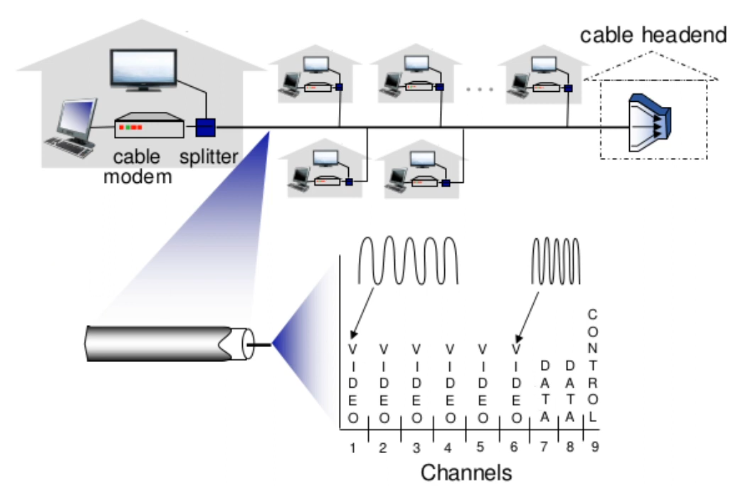
\includegraphics[width=0.6\textwidth]{img/cap-01/tv-a-cabo.png}
        \caption{Rede de acesso via TV a cabo (FDM).}
    \end{figure}

    \begin{figure}[H]
        \centering
        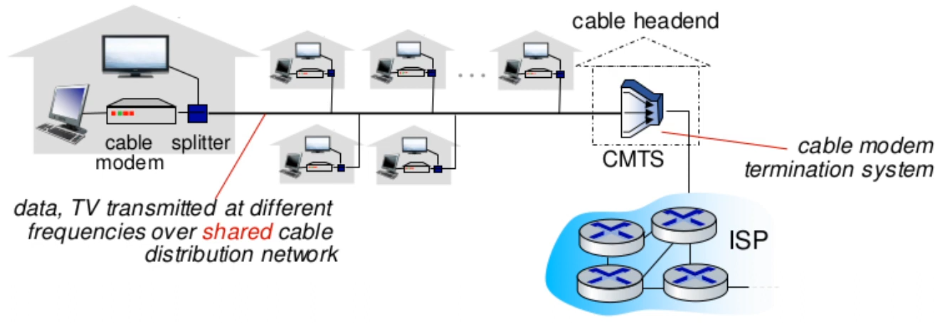
\includegraphics[width=0.6\textwidth]{img/cap-01/tv-a-cabo2.png}
        \caption{Arquitetura HFC híbrida coaxial-fibra.}
    \end{figure}

    \begin{itemize}
        \item Utiliza-se \textbf{HFC (Hybrid Fiber Coaxial)}, uma solução híbrida : \\
            $\hookrightarrow$ O \textbf{cabo coaxial} vai até o usuário. \\
            $\hookrightarrow$ A \textbf{interconexão} da rede é feita usando \textbf{fibra óptica}.
        \item \textbf{Assimétrica}: a capacidade de download e upload são diferentes.
        \item \textbf{Meio compartilhado}: o enlace é compartilhado entre vários usuários domésticos.
    \end{itemize}

    \paragraph{Rede baseada em DSL (\textit{Digital Subscriber Line})}
    \begin{itemize}
        \item Utiliza os \textbf{cabos telefônicos} como infraestrutura de enlace.
        \item A conexão \underline{não é compartilhada}.
        \item \textbf{Assimétrica} — download e upload possuem taxas diferentes.
    \end{itemize}

    \begin{figure}[H]
        \centering
        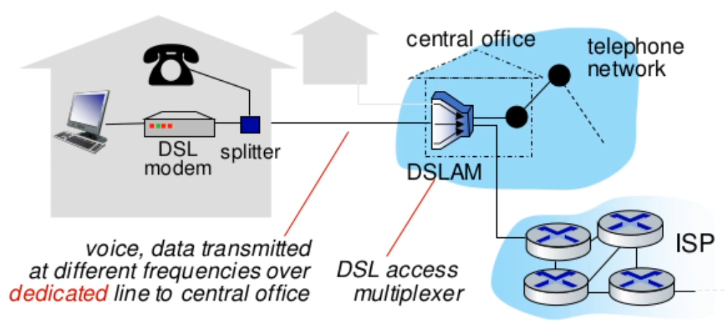
\includegraphics[width=0.6\textwidth]{img/cap-01/dsl.png}
        \caption{Rede DSL utilizando a infraestrutura telefônica.}
    \end{figure}

    {\textbf{Rede Doméstica}}

    \begin{figure}[H]
        \centering
        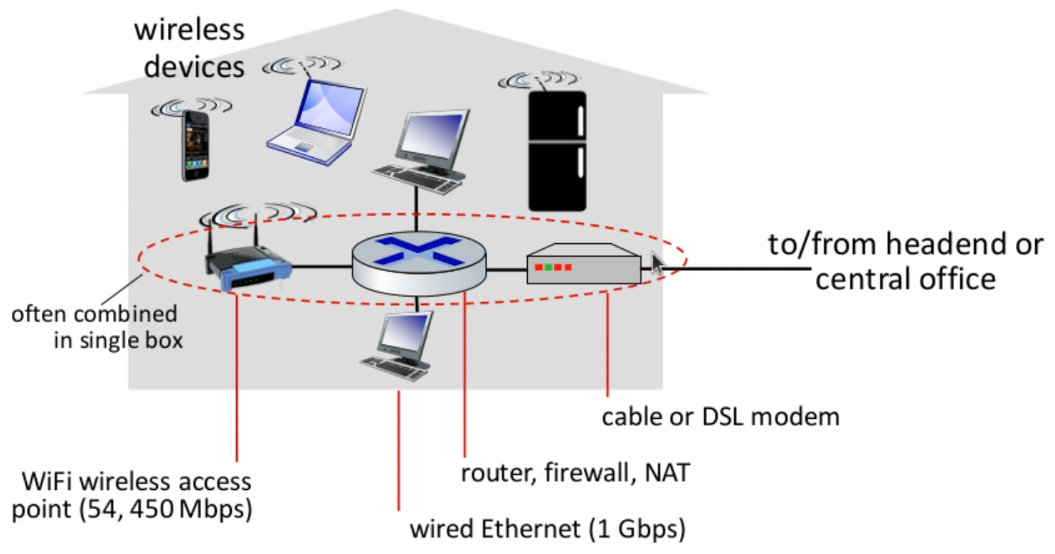
\includegraphics[width=0.6\textwidth]{img/cap-01/rede-domestica.png}
        \caption{Exemplo de rede doméstica.}
    \end{figure}

    \paragraph{Redes de Acesso Sem Fio (Wireless)}
    \begin{itemize}
        \item O \textbf{roteador de borda} é conectado a um \textbf{ponto de acesso}.
        \item \textbf{Locais}: alcance reduzido (domésticas, empresas) — \textbf{WiFi}.
        \item \textbf{Longas distâncias}: móveis (4G/5G), com pontos de acesso em \textbf{torres}, menor capacidade de transmissão.
    \end{itemize}

    \paragraph{Redes de Acesso Institucionais}
    \begin{itemize}
        \item Utilizadas em \textbf{universidades}, \textbf{empresas}, etc.
        \item Maior complexidade de interconexão — acesso sem fio conectado a switches e roteadores.
        \item Tecnologias utilizadas : \\
            $\hookrightarrow$ \textbf{Ethernet} \\
            $\hookrightarrow$ \textbf{WiFi}
    \end{itemize}

    \begin{figure}[H]
        \centering
        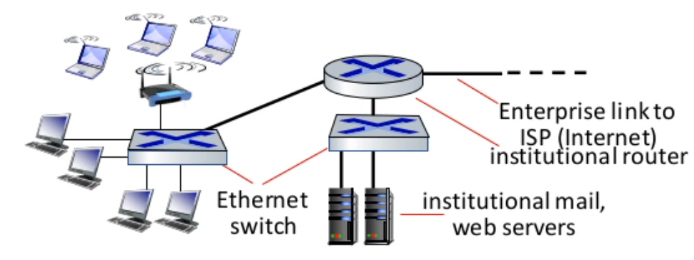
\includegraphics[width=0.6\textwidth]{img/cap-01/rede-institucional.png}
        \caption{Rede de acesso institucional.}
    \end{figure}

    \subsubsection*{Hosts (Sistemas Finais)}
    \begin{itemize}
        \item Quando o \textbf{host} tem conectividade, é possível enviar \textbf{pacotes de dados} até o destinatário.
        \item \textbf{Função de envio :} \\
            $\hookrightarrow$ Pega uma \textbf{mensagem} de uma aplicação.
            $\hookrightarrow$ Quebra essa mensagem em \textbf{pacotes menores} de tamanho $L$ bits.
            $\hookrightarrow$ Esses pacotes são transmitidos a uma taxa de transmissão $R$ (\textbf{bits/s}), correspondente à capacidade do enlace.
        \item \underline{Tempo de retardo (delay)} = tempo necessário para transmitir um pacote:  
        \[
        \text{delay} = \frac{L (\text{bits})}{R (\text{bits/s})}
        \]
    \end{itemize}

    \subsubsection*{Links (Enlaces)}
    \begin{itemize}
        \item Utilizados para a \textbf{interconexão de dispositivos}.
        \item Caracterizados por propriedades físicas.
        \item O \textbf{bit} é propagado entre transmissor e receptor.
        \item \textbf{Tipos de enlaces :} \\
            $\hookrightarrow$ \textbf{Guiados}: sinal se propaga em meio sólido (fibra óptica, cabos coaxiais, par trançado). \\
            \textbf{Não guiados}: sinal se propaga de forma livre (ondas eletromagnéticas). 
    \end{itemize}

    \paragraph{Cabos Par Trançado (Twisted Pair - TP)}
    
        $bullet$ Categorias mais comuns: \textbf{Cat 5}, \textbf{Cat 6}.
    
    \begin{figure}[H]
        \centering
        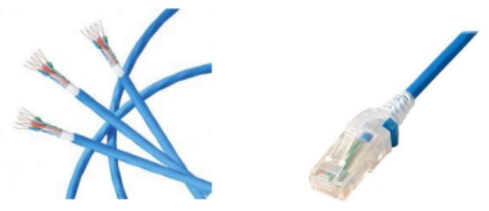
\includegraphics[width=0.6\textwidth]{img/cap-01/cabos-tp.png}
        \caption{Cabos Par Trançado (Twisted Pair).}
    \end{figure}

    \paragraph{Cabos Coaxiais}
    \begin{itemize}
        \item Dois condutores de cobre concêntricos.
        \item \textbf{Bidirecional}: transmite e recebe dados simultaneamente.
        \item Suporta \textbf{conexão de banda larga} — coexistência de múltiplas frequências no mesmo cabo.
    \end{itemize}

    \begin{figure}[H]
        \centering
        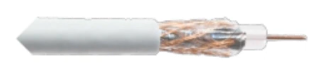
\includegraphics[width=0.6\textwidth]{img/cap-01/cabo-coaxial.png}
        \caption{Estrutura de um cabo coaxial.}
    \end{figure}

    \paragraph{Cabos de Fibra Óptica}
    \begin{itemize}
        \item Feitos de \textbf{vidro}.
        \item Transmissão em \textbf{alta velocidade} e \textbf{longa distância}.
        \item \textbf{Taxa de erro muito baixa}, dispensando regeneração do sinal.
        \item Imunes a \textbf{ruídos eletromagnéticos}.
    \end{itemize}

    \begin{figure}[H]
        \centering
        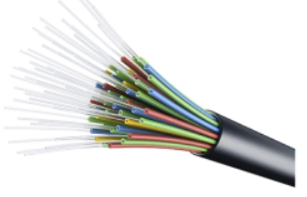
\includegraphics[width=0.6\textwidth]{img/cap-01/fibra-optica.png}
        \caption{Cabo de fibra óptica.}
    \end{figure}

    \paragraph{Transmissão via Rádio}
    \begin{itemize}
        \item Sinal transmitido no \textbf{espectro eletromagnético}.
        \item Comunicação \textbf{sem fio} e geralmente em modo \textbf{broadcast} (difusão).
        \item Operação \textbf{half-duplex}: alterna entre receber e enviar informações.
        \item \textbf{Problemas comuns de transmissão :} \\
            $\hookrightarrow$ Reflexão \\
            $\hookrightarrow$ Obstrução por objetos \\
            $\hookrightarrow$ Interferência 
        \item \textbf{Tipos de transmissão via rádio :} \\
            $\hookrightarrow$ Micro-ondas terrestres \\
            $\hookrightarrow$ \textbf{Wireless LAN} (WiFi) \\
            $\hookrightarrow$ \textbf{Sem fio de longo alcance} (4G/5G) \\
            $\hookrightarrow$ \textbf{Satélite} — possui \underline{retardo de transmissão elevado}.
    \end{itemize}

    \subsection{Núcleo da Rede}

    \begin{itemize}
        \item Parte \textbf{central da rede}, responsável por interconectar as redes de acesso.
        \item É composta por uma \textbf{malha de roteadores interconectados} que realizam o \textbf{encaminhamento de pacotes de dados} gerados pelos sistemas finais.
    \end{itemize}

    \subsubsection*{Comutação de Pacotes (\textit{Packet Switching})}
    \begin{itemize}
        \item O \textbf{sistema final} divide a \textbf{mensagem da aplicação} em \textbf{pacotes}.
        \item Esses pacotes são encaminhados \underline{roteador a roteador}, seguindo um caminho até o destino.
        \item Cada pacote é transmitido utilizando \textbf{toda a capacidade do enlace} entre os roteadores.
    \end{itemize}

    \begin{figure}[H]
        \centering
        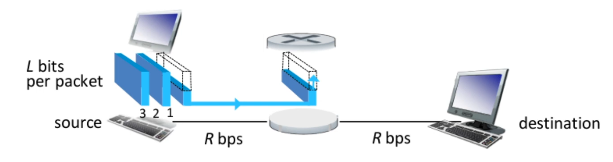
\includegraphics[width=0.55\textwidth]{img/cap-01/retardo.png}
        \caption{Encaminhamento de pacotes e retardo na transmissão.}
    \end{figure}

    \begin{itemize}
        \item Cada pacote passa por uma série de roteadores desde a origem até o destino.
        \item Em cada roteador é necessário que o pacote seja \textbf{recebido completamente} antes de ser retransmitido.
        \item \underline{Delay fim-a-fim}: $2L/R$ (assumindo delay de propagação nulo).
        \item \textbf{Exemplo:} $L = 10$ Kbits, $R = 100$ Mbps $\Rightarrow$ cada salto de transmissão leva $0.1$ ms.
    \end{itemize}

    \paragraph{Atrasos e Perdas (\textit{Queueing Delay, Loss})}
    \begin{itemize}
        \item Quando a \textbf{taxa de chegada} de pacotes em um roteador excede a \textbf{taxa de saída}, ocorre o \underline{enfileiramento}.
        \item Pacotes são \textbf{enfileirados} aguardando o enlace ficar livre — adicionando retardo ao processo de transmissão fim a fim.
        \item Caso a fila de saída esteja cheia, os pacotes são \textbf{descartados (perdidos)}.
    \end{itemize}

    \begin{figure}[H]
        \centering
        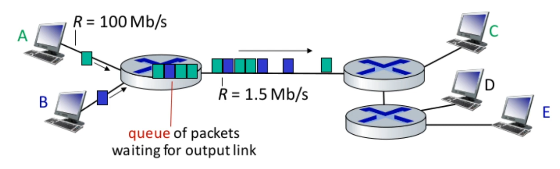
\includegraphics[width=0.55\textwidth]{img/cap-01/fila-e-perda.png}
        \caption{Fila de pacotes e perdas em roteadores.}
    \end{figure}

    \subsubsection*{Funções Principais do Núcleo da Rede}
    \begin{itemize}
        \item \textbf{Encaminhamento (Forwarding):} ação \underline{local} — move pacotes do enlace de entrada para o enlace de saída apropriado.
        \item \textbf{Roteamento (Routing):} ação \underline{global} — define os caminhos de origem a destino dentro da rede, utilizando \textbf{algoritmos de roteamento}.
    \end{itemize}

    \begin{figure}[H]
        \centering
        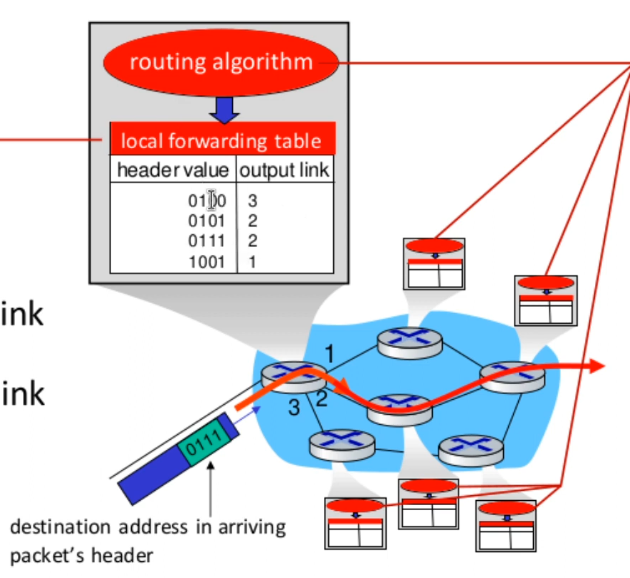
\includegraphics[width=0.55\textwidth]{img/cap-01/encaminhamento-roteamento.png}
        \caption{Diferença entre encaminhamento e roteamento.}
    \end{figure}

    \subsubsection*{Alternativa: Comutação por Circuito}
    \begin{itemize}
        \item Na comutação por circuito, existe uma \textbf{etapa inicial de conexão} onde : \\        
            $\hookrightarrow$ É definida a rota completa do início ao fim. \\
            $\hookrightarrow$ São \textbf{alocados recursos} nos roteadores ao longo do caminho. \\
            $\hookrightarrow$ Cada roteador envolvido armazena informação sobre essa rota. 
        \item Os pacotes transportam a informação sobre o \textbf{circuito virtual} ao qual pertencem.
    \end{itemize}

    \begin{figure}[H]
        \centering
        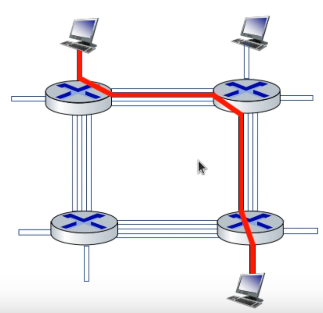
\includegraphics[width=0.55\textwidth]{img/cap-01/comutacao-circuitos.png}
        \caption{Comutação por circuito.}
    \end{figure}

    \paragraph{Técnicas de Multiplexação}
    \begin{itemize}
        \item \textbf{Frequency Division Multiplexing (FDM) :} \\
            $\hookrightarrow$ Divide a capacidade do enlace em \textbf{faixas de frequência}. \\
            $\hookrightarrow$ Cada faixa é dedicada a um usuário, transmitindo até a taxa máxima da sua banda.
        
        \begin{figure}[H]
            \centering
            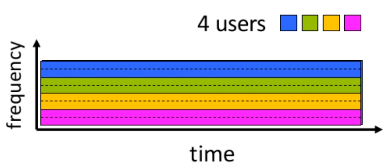
\includegraphics[width=0.55\textwidth]{img/cap-01/multiplexicacao-por-frequencia.png}
            \caption{Multiplexação por frequência (FDM).}
        \end{figure}

        \item \textbf{Time Division Multiplexing (TDM) :} \\
            $\hookrightarrow$ Divide o tempo de transmissão em \textbf{intervalos (slots)}. \\
            $\hookrightarrow$ Cada usuário transmite à taxa total do enlace durante o seu slot de tempo.
        
        \begin{figure}[H]
            \centering
            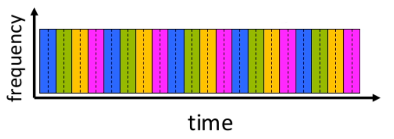
\includegraphics[width=0.55\textwidth]{img/cap-01/multiplexicacao-por-tempo.png}
            \caption{Multiplexação por tempo (TDM).}
        \end{figure}
    \end{itemize}

    \paragraph{Comparação: Comutação de Pacotes vs. Comutação de Circuitos}
    \begin{itemize}
        \item Ambas possuem a mesma \textbf{taxa de transmissão nominal}.
        \item A \textbf{comutação de pacotes} permite que mais usuários utilizem a rede simultaneamente.
        \item É mais eficiente para \textbf{“bursty data”} (rajadas de dados) : \\    
            $\hookrightarrow$ Melhor \textbf{compartilhamento de recursos}.
            $\hookrightarrow$ Operação mais \textbf{simples}, sem necessidade de estabelecimento de chamada.
        
        \item \textbf{Problema :} Ausência de controle de congestionamento. \\
            $\hookrightarrow$ Pode causar aumento de retardo e perda de pacotes devido ao transbordo das filas. \\
            $\hookrightarrow$ Protocolos específicos são utilizados para controle de congestionamento.
        
        \item Aplicações como \textbf{vídeo/áudio streaming} ainda utilizam comutação de circuitos.
    
    \end{itemize}

    \subsubsection*{Estrutura da Internet}
    \begin{itemize}
        \item Os \textbf{hosts} se conectam à Internet por meio de \textbf{provedores de acesso (ISPs)} : \\
            $\hookrightarrow$ Domésticos, empresariais ou institucionais.
        \item Esses provedores precisam se \textbf{interconectar} para permitir comunicação entre seus clientes.
        \item Isso resultou em uma rede de \textbf{alta complexidade}, moldada por \textbf{decisões econômicas e políticas}.
    \end{itemize}

    \begin{figure}[H]
        \centering
        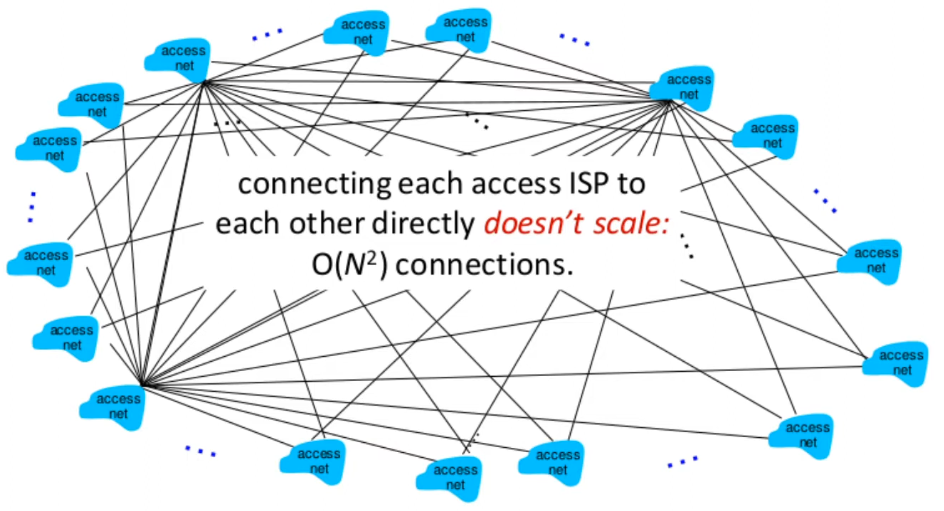
\includegraphics[width=0.55\textwidth]{img/cap-01/infraestrutura1.png}
        \caption{Evolução da infraestrutura da Internet.}
    \end{figure}

    \paragraph{Hierarquização da Conexão}
    \begin{itemize}
        \item Solução: criar um \textbf{provedor de acesso global}.
        \item Provedores locais se conectam a ele, estabelecendo uma relação \textbf{econômica} (pagamento pelo uso do serviço de trânsito).
    \end{itemize}

    \begin{figure}[H]
        \centering
        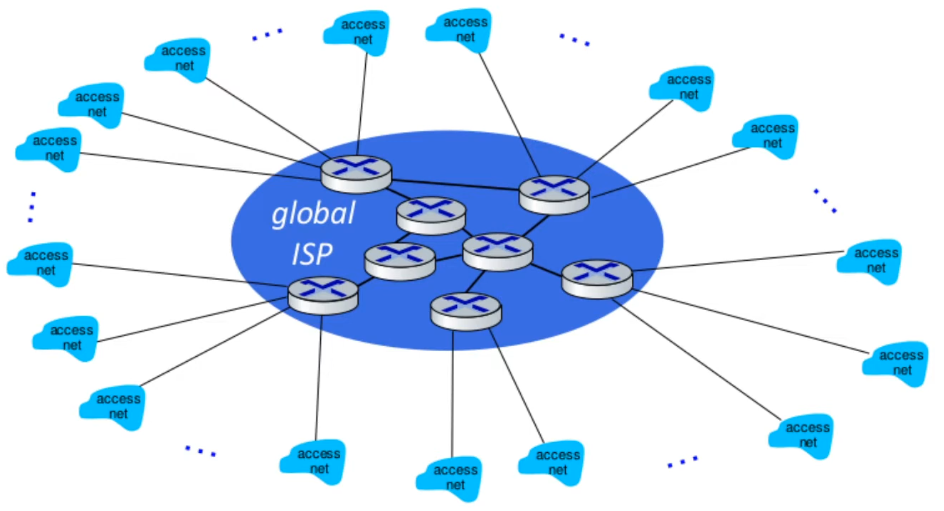
\includegraphics[width=0.55\textwidth]{img/cap-01/infraestrutura2.png}
        \caption{Conexão hierárquica entre provedores locais e globais.}
    \end{figure}

    \begin{itemize}
        \item Com o tempo, surgiu \textbf{concorrência} tanto por questões econômicas quanto geográficas.
    \end{itemize}

    \begin{figure}[H]
        \centering
        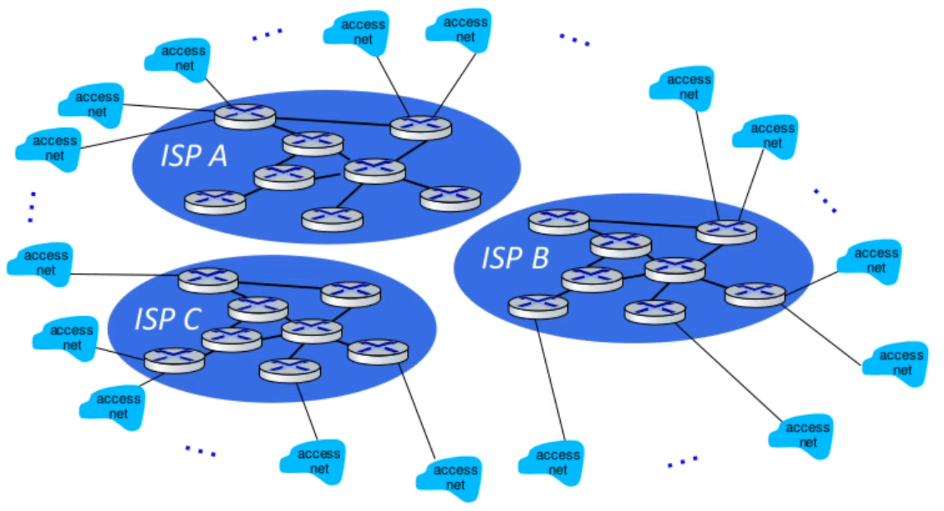
\includegraphics[width=0.55\textwidth]{img/cap-01/infraestrutura3.png}
        \caption{Concorrência e distribuição geográfica de provedores.}
    \end{figure}

    \paragraph{Peering e Pontos de Troca de Tráfego}
    \begin{itemize}
        \item A conexão entre provedores locais ocorre por meio de : \\
            $\hookrightarrow$ \textbf{Peering físico (peering link)} \\
            $\hookrightarrow$ \textbf{Pontos de Troca de Tráfego (IXP)}
    \end{itemize}

    \begin{figure}[H]
        \centering
        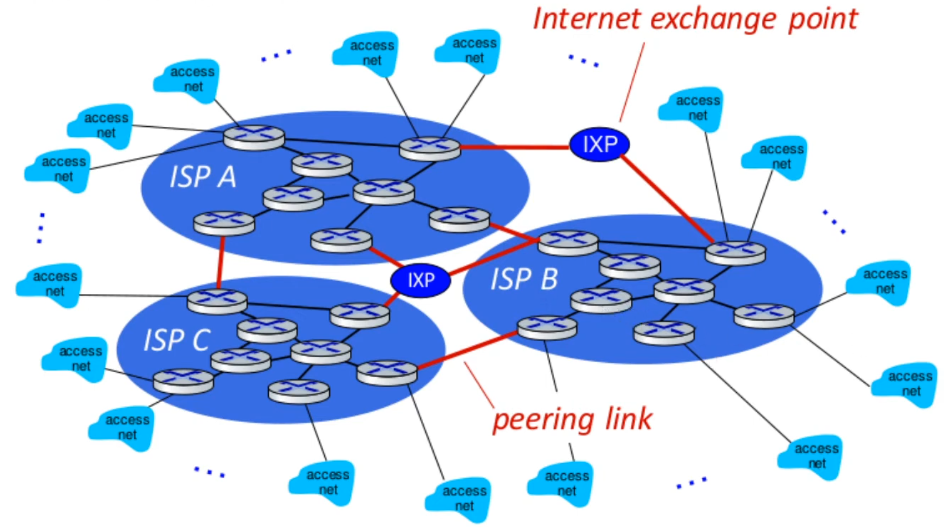
\includegraphics[width=0.55\textwidth]{img/cap-01/infraestrutura4.png}
        \caption{Conexão entre provedores locais e IXP.}
    \end{figure}

    \paragraph{Provedores Regionais e Globais}
    \begin{itemize}
        \item Devido à distância geográfica entre provedores globais e locais, surgiram \textbf{provedores regionais}.
        \item Grandes provedores de conteúdo (\textbf{Google, Microsoft, etc.}) se conectam diretamente aos provedores globais.
    \end{itemize}

    \begin{figure}[H]
        \centering
        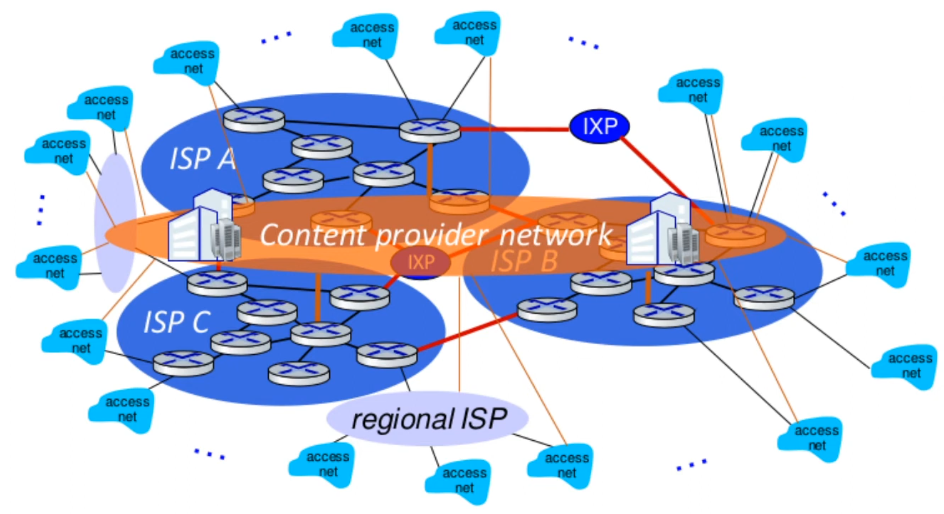
\includegraphics[width=0.55\textwidth]{img/cap-01/infraestrutura5.png}
        \caption{Conexão de provedores de conteúdo com provedores globais.}
    \end{figure}

    \paragraph{Hierarquia da Internet}
    \begin{figure}[H]
        \centering
        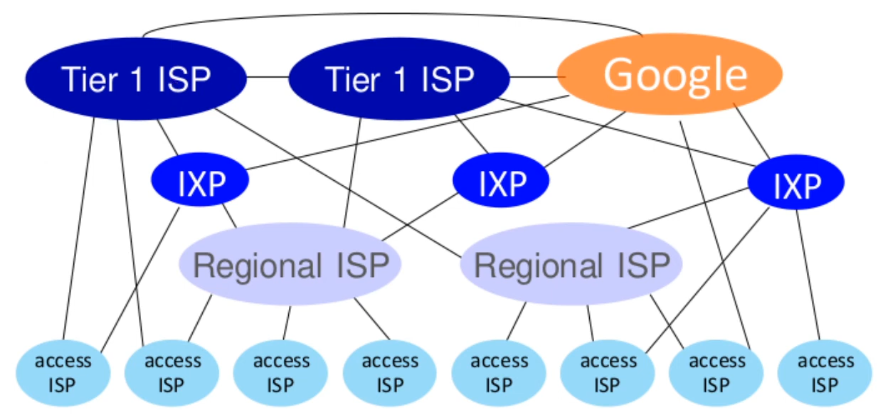
\includegraphics[width=0.55\textwidth]{img/cap-01/hierarquia.png}
        \caption{Hierarquia dos provedores de acesso à Internet.}
    \end{figure}

   \subsection{Performance}

    \begin{itemize}
        \item \textbf{Como ocorre a perda e o retardo de pacotes ?} \\
            $\hookrightarrow$ Pacotes enfileirados esperam a sua vez de serem transmitidos. \\
            $\hookrightarrow$ \textbf{Retardo de enfileiramento}: \underline{tempo que um pacote aguarda na fila} para ser transmitido. \\
            $\hookrightarrow$ \textbf{Retardo de transmissão}: \underline{tempo que leva para transmitir os bits} no enlace. \\
            $\hookrightarrow$ Se a \textbf{taxa de chegada} no enlace (temporariamente) excede a capacidade de saída, ocorre a \textbf{perda de pacotes}. 
      

        \begin{center}
            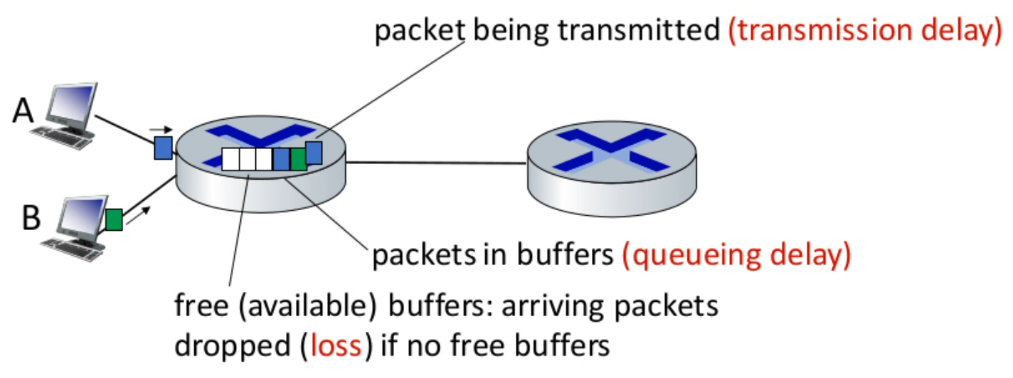
\includegraphics[width=0.6\textwidth]{img/cap-01/delay1.png}
        \end{center}

        \item \textbf{Retardo do Pacote: 4 Causas}
            $\hookrightarrow$ O retardo ocorre a cada nó (ou salto) na rede : 
            \[
            d_{nodal} = d_{proc} + d_{queue} + d_{trans} + d_{prop}
            \]
        

        \begin{center}
            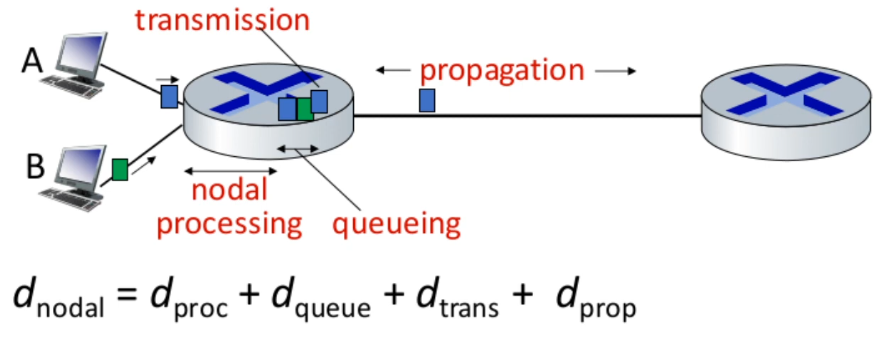
\includegraphics[width=0.7\textwidth]{img/cap-01/delay2.png}
        \end{center}

        \item \textbf{Componentes do Retardo :}
        
            $\hookrightarrow$ \textbf{$d_{proc}$ — Retardo de Processamento do Nó :}
            \begin{itemize}
                \item Tempo gasto pelo roteador para processar o pacote que acabou de chegar.
                \item Envolve tarefas como:
                \begin{itemize}
                    \item Conferir a integridade do pacote.
                    \item Verificar o endereço de saída do pacote.
                \end{itemize}
                \item Geralmente menor que 1 ms.
            \end{itemize}

            $\hookrightarrow$ \textbf{$d_{queue}$ — Retardo de Enfileiramento :}
            \begin{itemize}
                \item Tempo que o pacote aguarda na fila antes da transmissão.
                \item Depende do \textbf{nível de congestionamento} no roteador.
            \end{itemize}

            $\hookrightarrow$ \textbf{$d_{trans}$ — Retardo de Transmissão :}
            \begin{itemize}
                \item Tempo necessário para transmitir um pacote no enlace.
                \item Dados:
                \[
                L = \text{tamanho do pacote (bits)}, \quad R = \text{taxa de transmissão (bps)}
                \]
                \item Fórmula:
                \[
                d_{trans} = \frac{L}{R}
                \]
            \end{itemize}

            $\hookrightarrow$ \textbf{$d_{prop}$ — Retardo de Propagação :}
            \begin{itemize}
                \item Tempo necessário para que os bits do pacote \underline{propaguem até o destino}.
                \[
                d = \text{comprimento do enlace}, \quad s = \text{velocidade de propagação} \approx 2 \times 10^8 \text{ m/s}
                \]
                \item Fórmula:
                \[
                d_{prop} = \frac{d}{s}
                \]
            \end{itemize}
        
        \item \textbf{Exemplo: Caravanas de Carros}
        
            $\hookrightarrow$ Analogia :
            \begin{itemize}
                \item \textbf{1 Carro} $\rightarrow$ 1 \textbf{bit}.
                \item \textbf{Caravana} $\rightarrow$ \textbf{pacote}.
                \item \textbf{Pedágio} $\rightarrow$ \textbf{roteador}.
                \item \textbf{Estrada} $\rightarrow$ \textbf{enlace}.
            \end{itemize}
            
            $\hookrightarrow$ O pedágio leva 12 s para atender cada carro (tempo de transmissão). \\
            $\hookrightarrow$ A estrada tem pedágios a cada 100 km. \\
            $\hookrightarrow$ Um carro se propaga a 100 km/h. \\
            $\hookrightarrow$ \textbf{Pergunta 1:} Quanto tempo levaria para a caravana de 10 carros chegar ao 2º pedágio ? 
            
            \begin{itemize}
                \item Tempo de transmissão: $12 \times 10 = 120$ s.
                \item Tempo de propagação: $100$ km / $100$ km/h = 1 h.
                \item Tempo total: \textbf{62 minutos}.
            \end{itemize}
            $\hookrightarrow$ \textbf{Pergunta 2:} Se os carros se propagam a 1000 km/h e o pedágio leva 1 min por carro?
            \begin{itemize}
                \item Tempo de propagação: 6 min.
                \item O primeiro carro chega ao segundo pedágio após 7 min, antes de todos terminarem no primeiro pedágio.
            \end{itemize}
        \end{itemize}

        \begin{center}
            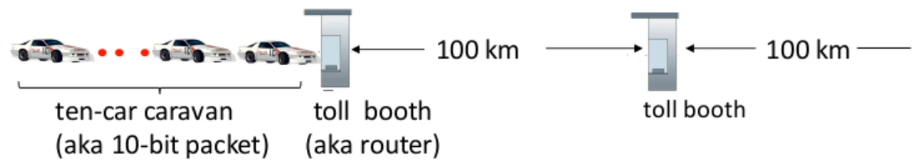
\includegraphics[width=0.7\textwidth]{img/cap-01/carro-pedagio.png}
        \end{center}

        $\hookrightarrow$ \textbf{Revisão: Retardo de Enfileiramento}
        
        $R = \text{Capacidade de transmissão (bps)}$ \\ 
        $L = \text{Tamanho do pacote (bits)}$ \\
        $a = \text{Taxa de chegada (pacotes/s)}$
        
        \begin{itemize}
            \item $La/R \approx 0$: retardo pequeno.
            \item $La/R \rightarrow 1$: retardo grande.
            \item $La/R > 1$: \underline{taxa de chegada maior que a capacidade de transmissão}, retardo tende ao infinito.
        \end{itemize}

        \begin{center}
            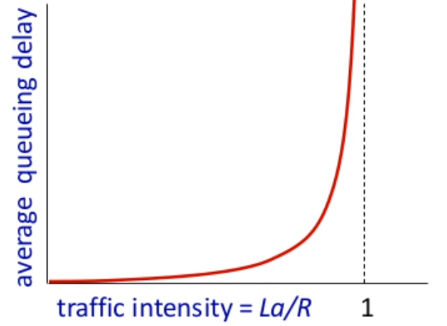
\includegraphics[width=0.6\textwidth]{img/cap-01/retardo-de-enfileiramento.png}
        \end{center}

        $\hookrightarrow$ \textbf{Exemplo Real — \texttt{traceroute}}
        \begin{itemize}
            \item Programa que permite \underline{avaliar cada roteador} ao longo da rota seguida pelos pacotes.
            \item Mostra o \textbf{tempo de ida e volta (RTT)} de cada salto.
        \end{itemize}

        \begin{center}
            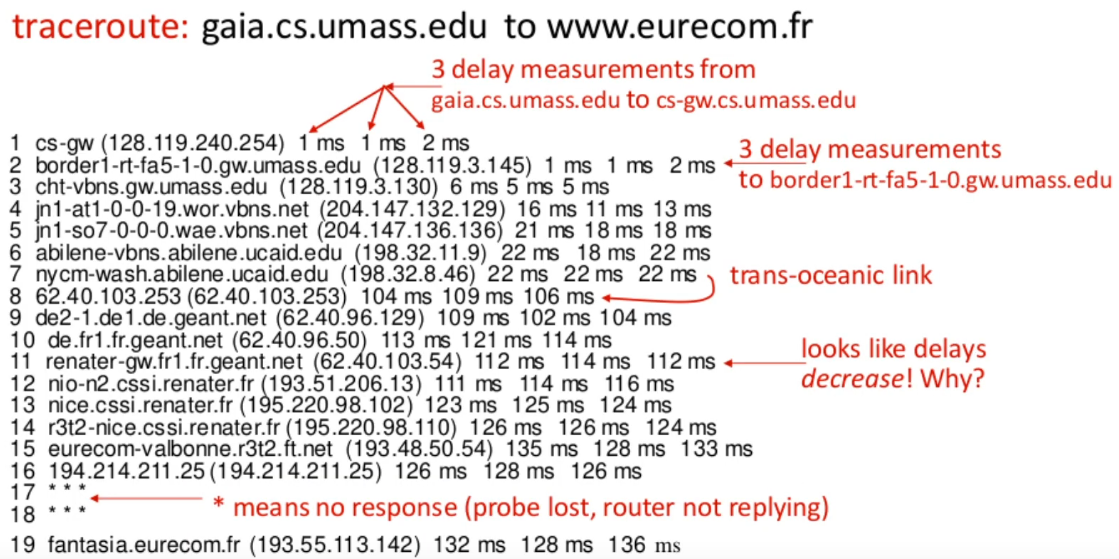
\includegraphics[width=0.7\textwidth]{img/cap-01/traceroute-exemplo.png}
        \end{center}

        $\hookrightarrow$ \textbf{Perda de Pacotes}
        \begin{itemize}
            \item A fila (\textbf{buffer}) precede um enlace de saída.
            \item Quando a fila está cheia, o pacote é \underline{descartado}.
            \item Pacotes perdidos precisam ser \textbf{retransmitidos}.
        \end{itemize}

        \begin{center}
            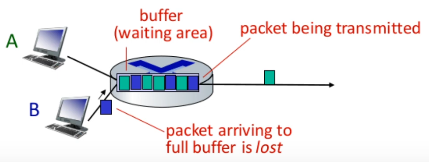
\includegraphics[width=0.6\textwidth]{img/cap-01/perda-de-pacotes.png}
        \end{center}

        $\hookrightarrow$ \textbf{Vazão (Throughput)}
        \begin{itemize}
            \item \textbf{Throughput}: \underline{taxa de transmissão efetiva} percebida por uma conexão.
            \item Tipos:
            \begin{itemize}
                \item \textbf{Instantânea}: medida em um determinado instante.
                \item \textbf{Média}: média ao longo de um período.
            \end{itemize}
            \item A vazão é sempre limitada pelo \textbf{link gargalo}.
        \end{itemize}

        \begin{center}
            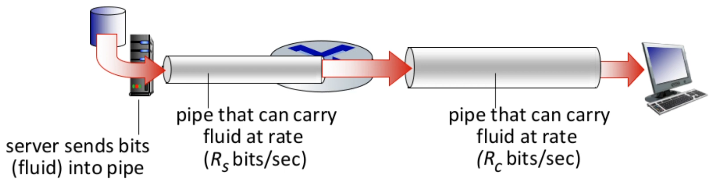
\includegraphics[width=0.6\textwidth]{img/cap-01/vazao.png}
        \end{center}

        \begin{center}
            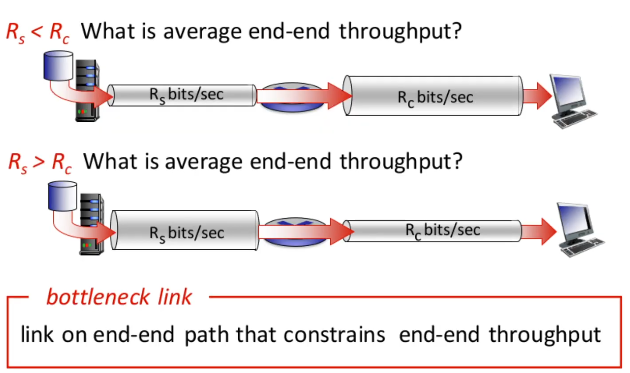
\includegraphics[width=0.6\textwidth]{img/cap-01/exemplo-vazao.png}
        \end{center}

        \begin{center}
            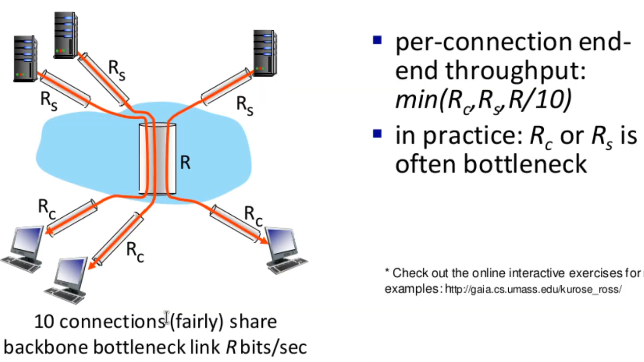
\includegraphics[width=0.6\textwidth]{img/cap-01/exemplo-vazao2.png}
        \end{center}

    \subsection{Camadas de Protocolos e Modelos de Serviços}

    \begin{itemize}
        \item \textbf{Questão inicial:} Existia alguma maneira de organizar a estrutura da Internet?

        \item \textbf{Exemplo: Organização para Viajar de Avião} \\
            $\hookrightarrow$ Uma viagem de avião envolve uma série de etapas e serviços distintos. \\
            $\hookrightarrow$ Cada etapa pode ser vista como uma \textbf{camada}, responsável por uma parte específica do processo.
        

        \begin{figure}[H]
            \centering
            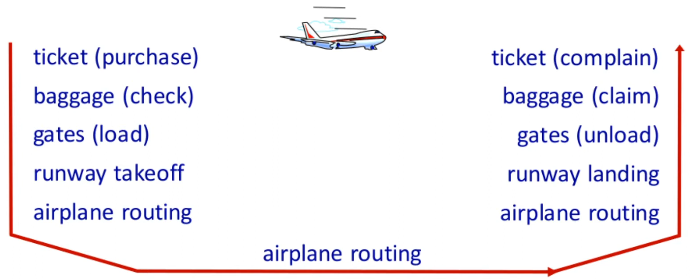
\includegraphics[width=0.6\textwidth]{img/cap-01/exemplo-aviao.png}
            \caption{Organização em etapas de uma viagem de avião.}
        \end{figure}

        \item \textbf{Camadas :} \\ 
            $\hookrightarrow$ Cada camada implementa um \textbf{serviço} específico. \\
            $\hookrightarrow$ Cada camada tem uma \textbf{contrapartida} tanto na origem quanto no destino.
        
        \begin{figure}[H]
            \centering
            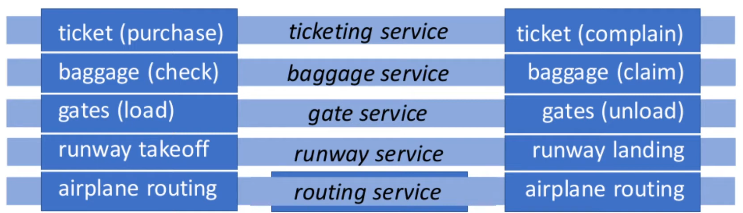
\includegraphics[width=0.6\textwidth]{img/cap-01/exemplo-aviao2.png}
            \caption{Camadas de serviço e suas contrapartidas.}
        \end{figure}

        \item \textbf{Por que usar camadas ?} \\
            $\hookrightarrow$ A ideia surge naturalmente em sistemas complexos. \\
            $\hookrightarrow$ \textbf{Abstrai} partes do sistema em diferentes camadas. \\
            $\hookrightarrow$ Cada camada deve ser \textbf{bem definida} e possuir uma \textbf{interface clara}. \\
            $\hookrightarrow$ Facilita a \textbf{modularização}, \textbf{manutenção} e \textbf{atualização} do sistema. \\
            $\hookrightarrow$ \underline{Problema:} pode haver \textbf{redundância de ações} entre camadas.

        \item \textbf{Pilha de Protocolos da Internet (TCP/IP)}
        
            $\hookrightarrow$ \textbf{Aplicação :} Suporta as aplicações que estão executando nos sistemas finais.
            \begin{itemize}
                \item Exemplos: \texttt{HTTP}, \texttt{SMTP}, \texttt{IMAP}.
            \end{itemize}
            
            $\hookrightarrow$ \textbf{Transporte :} Responsável pela \textbf{transferência de pacotes entre processos} que estão executando nos sistemas finais.
            \begin{itemize}
                \item Exemplos: \texttt{UDP}, \texttt{TCP}.
            \end{itemize}

            $\hookrightarrow$ \textbf{Rede :} Faz o \textbf{roteamento dos pacotes} da origem até o destino.
            \begin{itemize}
                \item Exemplos: \texttt{IP}, \texttt{Protocolos de roteamento}.
            \end{itemize}

            $\hookrightarrow$ \textbf{Enlace :} Garante a \textbf{transferência de dados entre dispositivos diretamente conectados}.
            \begin{itemize}
                \item Exemplos: \texttt{Ethernet}, \texttt{802.11 (WiFi)}, \texttt{PPP}.
            \end{itemize}

            $\hookrightarrow$ \textbf{Física :} Responsável pela \textbf{transmissão dos bits} através do meio físico.
        

        \begin{center}
            \begin{tikzpicture}
                \node[draw, minimum width=4cm, minimum height=1cm, fill=blue!10] (app) {\textbf{Aplicação}};
                \node[draw, below=0cm of app, minimum width=4cm, minimum height=1cm, fill=green!10] (transp) {\textbf{Transporte}};
                \node[draw, below=0cm of transp, minimum width=4cm, minimum height=1cm, fill=yellow!10] (rede) {\textbf{Rede}};
                \node[draw, below=0cm of rede, minimum width=4cm, minimum height=1cm, fill=orange!10] (enlace) {\textbf{Enlace}};
                \node[draw, below=0cm of enlace, minimum width=4cm, minimum height=1cm, fill=red!10] (fisica) {\textbf{Física}};
            \end{tikzpicture}
        \end{center}

        \item \textbf{Encapsulamento :} \\
            $\hookrightarrow$ Cada camada adiciona seu próprio cabeçalho à unidade de dados recebida da camada superior. \\
            $\hookrightarrow$ O processo é \textbf{reverso} no destino: cada camada remove seu cabeçalho correspondente. \\
            $\hookrightarrow$ Esse mecanismo garante que cada camada só interaja com sua correspondente no outro sistema.
        
        \begin{figure}[H]
            \centering
            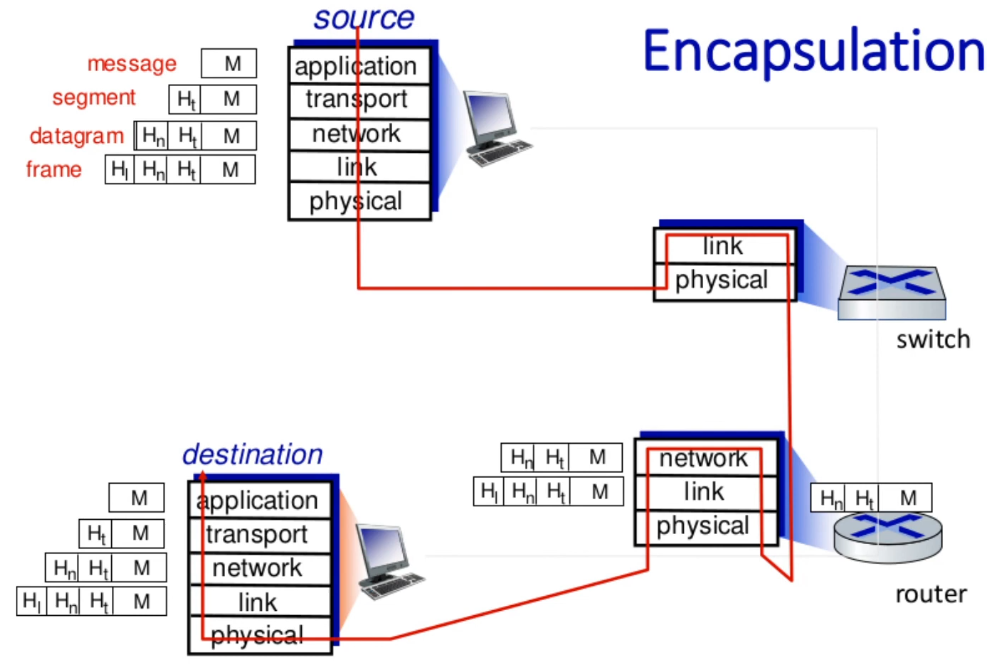
\includegraphics[width=0.65\textwidth]{img/cap-01/encapsulamento.png}
            \caption{Processo de encapsulamento nas camadas de protocolos.}
        \end{figure}
    \end{itemize}

\section{Camada de Aplicação}

\section{Camada de Transporte}

\section{Camada de Redes}

    \subsection{Introdução}

        \begin{itemize}[left=0.5cm, align=left, nosep]
            \item \textbf{Função principal:} fornece o transporte de segmentos dos hospedeiros de origem até os hospedeiros de destino. \\        
                $\hookrightarrow$ \textbf{Transmissor:} encapsula os segmentos em datagramas e encaminha para a camada de enlace; \\
                $\hookrightarrow$ \textbf{Receptor:} entrega os segmentos ao protocolo da camada de transporte.
        \end{itemize}

        \begin{center}
            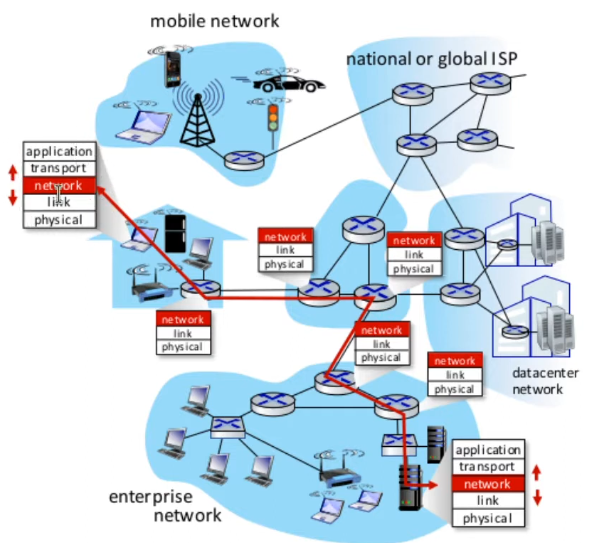
\includegraphics[width=0.65\textwidth]{img/cap-04/camada-de-redes-introd.png}
        \end{center}

        \begin{itemize}[left=0.5cm, align=left, nosep]
            \item A camada de redes deve estar implementada em todos os dispositivos ao longo da rota entre origem e destino.
        \end{itemize}

        \subsubsection*{Roteadores}
            \begin{itemize}[left=0.5cm, align=left, nosep]
            \item \textbf{Função :} \\
                $\hookrightarrow$ Examinar os cabeçalhos dos datagramas IP para extrair o endereço de destino; \\
                $\hookrightarrow$ Decidir para qual interface de saída o pacote será encaminhado.
            \end{itemize}

        \subsubsection*{Funções Principais da Camada de Rede}
            \begin{itemize}[left=0.5cm, align=left, nosep]
                \item \textbf{Encaminhamento:} move pacotes de uma interface de entrada para a interface de saída apropriada;
                \item \textbf{Roteamento:} determina a rota da origem até o destino (definida por algoritmos de roteamento).
            \end{itemize}

            \textbf{Analogia:} Fazer uma viagem
            \begin{itemize}[left=0.5cm, align=left, nosep]
                \item \textbf{Encaminhamento:} decisão tomada em cada encruzilhada;
                \item \textbf{Roteamento:} processo de definir todo o caminho de origem até o destino.
            \end{itemize}

            \begin{center}
                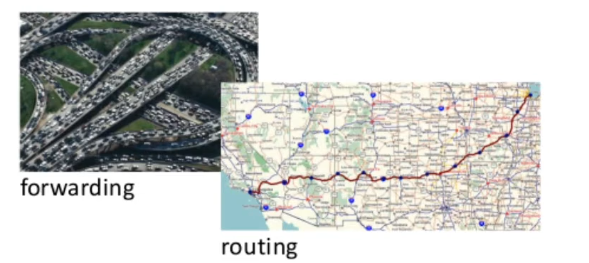
\includegraphics[width=0.55\textwidth]{img/cap-04/viagem.png}
            \end{center}

        \subsubsection*{Plano de Dados}
            \begin{itemize}[left=0.5cm, align=left, nosep]
                \item Local por dispositivo, função implementada por roteador;
                \item Ao receber um datagrama, o roteador analisa o cabeçalho e decide o encaminhamento.
            \end{itemize}

            \begin{center}
                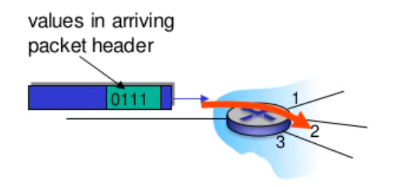
\includegraphics[width=0.65\textwidth]{img/cap-04/plano-de-dados.png}
            \end{center}

        \subsubsection*{Plano de Controle}
            \begin{itemize}[left=0.5cm, align=left, nosep]
                \item Lógica de toda a rede, determinando como datagramas são roteados de origem até destino;
                \item Implementações possíveis:
                
                \begin{enumerate}[left=0.5cm, align=left, nosep]
                    
                    \item \textbf{Algoritmos tradicionais de roteamento :} \\
                        $\hookrightarrow$ Implementados nos roteadores; \\
                        $\hookrightarrow$ Cada roteador executa uma parte do algoritmo de forma distribuída.
                    
                    \begin{center}
                        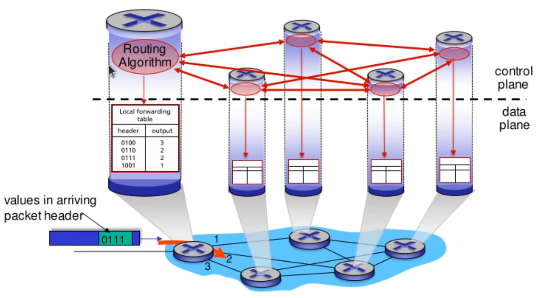
\includegraphics[width=0.6\textwidth]{img/cap-04/algorimo-roteamento.png}
                    \end{center}
                    
                    \item \textbf{SDN (Software Defined Networking) :} \\
                        $\hookrightarrow$ Implementado em controladores remotos; \\
                        $\hookrightarrow$ Controladores calculam e instalam as tabelas de encaminhamento nos roteadores.
                    
                    \begin{center}
                        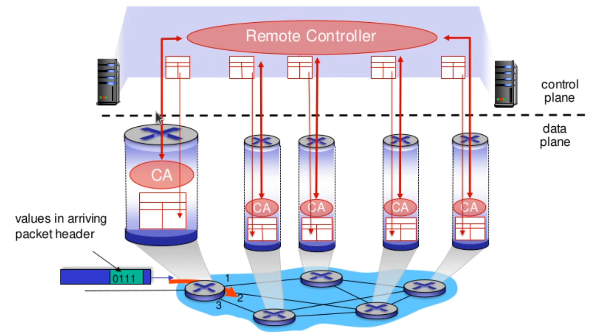
\includegraphics[width=0.6\textwidth]{img/cap-04/sdn.png}
                    \end{center}
                
                \end{enumerate}

            \end{itemize}

        \subsubsection*{Modelo de Serviço de Redes para Datagramas}
            \begin{itemize}[left=0.5cm, align=left, nosep]
                \item \textbf{Serviços para datagramas individuais :} \\
                    $\hookrightarrow$ Garantia de entrega; \\
                    $\hookrightarrow$ Garantia de entrega com atraso menor que 40 ms; \\
                    $\hookrightarrow$ Garantia de integridade; \\
                    $\hookrightarrow$ Garantia de confiabilidade.
                \item \textbf{Serviços para fluxos de datagramas :}
                    $\hookrightarrow$ Entrega em ordem; \\
                    $\hookrightarrow$ Garantia de taxa mínima de transferência; \\
                    $\hookrightarrow$ Restrição de variação de atraso (jitter).
            \end{itemize}

        \textbf{Modelo da Internet:} \textit{"Best Effort"} — não há garantias de entrega, temporização, ordenação ou taxa mínima de transmissão.

        \begin{table}[h!]
            \centering
            \renewcommand{\arraystretch}{1.3}
            \setlength{\tabcolsep}{3pt}
            \arrayrulecolor{blue}
            \begin{tabular}{|c|c|cccc|}
                \hline
                \textbf{Network Architecture} & \textbf{Service Model} &
                \multicolumn{4}{c|}{\textbf{Quality of Service (QoS) Guarantees?}} \\ \cline{3-6}
                & & \textbf{Bandwidth} & \textbf{Loss} & \textbf{Order} & \textbf{Timing} \\ \hline
                Internet & best effort & none & no & no & no \\ \hline
                ATM & Constant Bit Rate & Constant rate & yes & yes & yes \\ \hline
                ATM & Available Bit Rate & Guaranteed min & no & yes & no \\ \hline
                Internet & Intserv (RFC 1633) & yes & yes & yes & yes \\ \hline
                Internet & Diffserv (RFC 2475) & possible & possibly & possibly & no \\ \hline
            \end{tabular}
            \caption{Comparação de garantias de QoS entre diferentes arquiteturas e modelos de serviço.}
        \end{table}

        \subsubsection*{Reflexões sobre o Serviço “Best Effort”}
            \begin{itemize}[left=0.5cm, align=left, nosep]
                \item A simplicidade do mecanismo permitiu o crescimento da Internet;
                \item Na prática, há \textbf{superprovisionamento} de recursos para evitar congestionamentos;
                \item Há múltiplos mecanismos de \textbf{replicação e distribuição de conteúdo}, mantendo dados próximos dos usuários;
                \item Muitos serviços replicam conteúdo localmente, inclusive no provedor de acesso;
                \item O controle de congestionamento é eficiente em \textbf{serviços elásticos} — aplicações que usam toda a banda disponível.
            \end{itemize}

    \subsection{O tem dentro de um roteador ?}
        
        \begin{itemize}[left=0.5cm, align=left, nosep]
            \item \textbf{Arquitetura geral de um roteador :}
        
            \begin{center}
                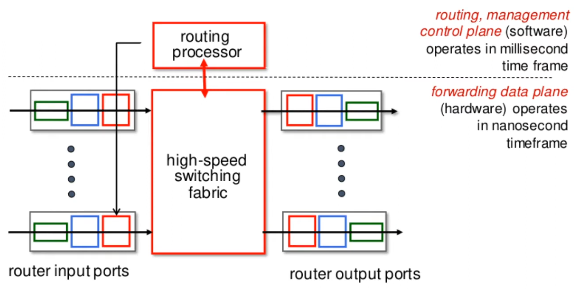
\includegraphics[width=0.65\textwidth]{img/cap-04/arquitetura-geral-roteador.png}
            \end{center}

            \item \textbf{Porta de Entrada :}
            
            \begin{center}
                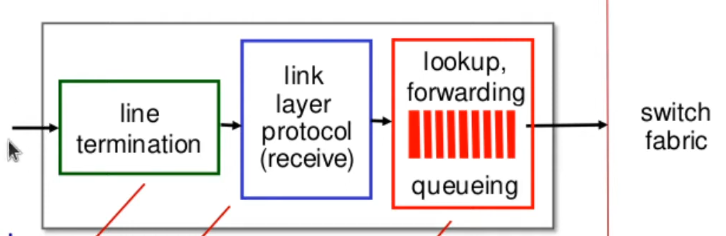
\includegraphics[width=0.55\textwidth]{img/cap-04/porta-de-entrada.png}
            \end{center}
            
            \item \textbf{Caixa Verde (Camada Física):} recepção dos bits;
            \item \textbf{Azul (Camada de Enlace):} Ethernet;
            \item \textbf{Vermelho:} operações de checagem do endereço de destino do pacote (lookup); \\
                $\hookrightarrow$ Objetivo da interface: encaminhar o pacote para a matriz de comutação na velocidade de linha; \\
                $\hookrightarrow$ Enfileiramento dos pacotes para evitar perdas em caso de chegada de datagramas for superior à capacidade \\
                $\hookrightarrow$ Decisão de encaminhamento :
                \begin{itemize}
                    \item Tradicional: Encaminhamento é baseado somente no endereço de IP do destino contido no cabeçalho;
                    \item Generalizado: Encaminhamento é baseado em qualquer informação contida no cabeçalho do datagrama
                \end{itemize}
            
        \end{itemize}

        \subsubsection*{Decisão de Encaminhamento :} 
    
            \begin{itemize}[left=0.5cm, align=left, nosep]
                \item O roteador possui uma tabela de encaminhamento que referencia endereços de destino e indica a interface de saída correspondente.
            
                \begin{center}
                    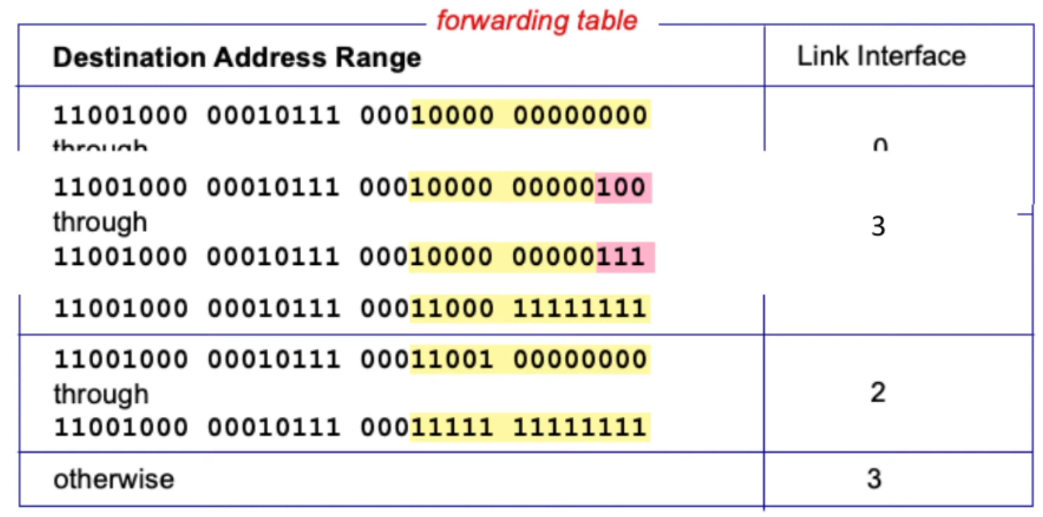
\includegraphics[width=0.65\textwidth]{img/cap-04/tabela-de-encaminhamento.png}
                \end{center}

                \item \textbf{Casamento de maior prefixo:} busca o endereço que melhor coincide com o endereço de destino do pacote na tabela.
            
                \begin{table}[h!]
                    \centering
                    \renewcommand{\arraystretch}{1.2}
                    \setlength{\tabcolsep}{6pt}
                    \arrayrulecolor{blue}

                    \begin{tabular}{|l|c|}
                        \hline
                        \textbf{Destination Address Range} & \textbf{Link Interface} \\ \hline
                        11001000 00010111 00010*** ******** & 0 \\ \hline
                        11001000 00010111 00011000 ******** & 1 \\ \hline
                        11001000 00010111 00011*** ******** & 2 \\ \hline
                        \textit{otherwise} & 3 \\ \hline
                    \end{tabular}

                    \caption{Tabela de encaminhamento com faixas de endereços de destino e interfaces de saída.}
                \end{table} 

                \textbf{\textcolor{blue}{Examples:}} \\[2pt]
                \texttt{11001000 00010111 00010110 10100001} \quad \textcolor{blue}{which interface? 1 } \\
                \texttt{11001000 00010111 00011000 10101010} \quad \textcolor{blue}{which interface? 2 }

                \item Geralmente, usa-se alta performance com TCAMs (memória ternária de conteúdo), permitindo o casamento em apenas um ciclo de clock.

            \end{itemize}

        \subsubsection*{Matrizes de Comutação} 

            \begin{itemize}[left=0.5cm, align=left, nosep]
                \item Transportam pacotes da interface de entrada até a interface de saída apropriada
                \item \textbf{Taxa de comutação :} Velocidade com que pacotes podem ser transferidos das entradas para as saídas \\
                    $\hookrightarrow$ Frequentemente medida como múltiplo da taxa de linha de entrada/saída; \\
                    $\hookrightarrow$ Taxa ideal = $N \times R$ (onde $N$ = número de entradas e $R$ = taxa dos enlaces das interfaces).
                    
                \begin{center}
                    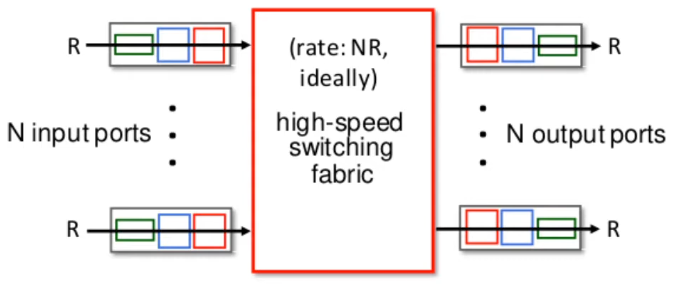
\includegraphics[width=0.65\textwidth]{img/cap-04/taxa-de-comutacao.png}
                \end{center}

                \item \textbf{Formas de implementação :}
                \begin{center}
                    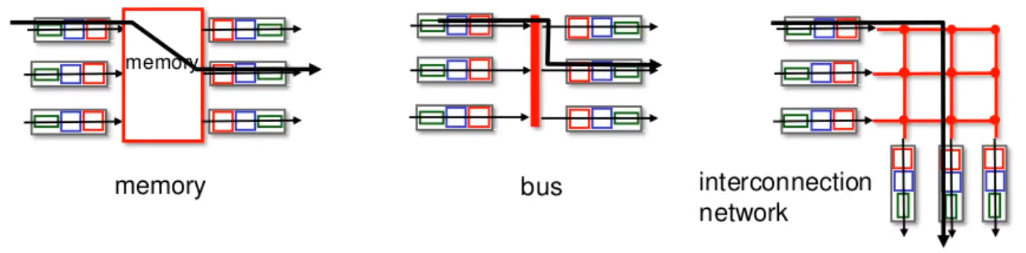
\includegraphics[width=0.65\textwidth]{img/cap-04/implementacao-matriz-de-comutacao.png}
                \end{center}

                \item \textbf{Memória :} \\ 
                    $\hookrightarrow$ Roteadores da primeira geração \\
                    $\hookrightarrow$ Usam computador tradicional com duas placas de rede \\
                    $\hookrightarrow$ Pacote é copiado para a memória do sistema antes do encaminhamento \\
                    $\hookrightarrow$ Problemas :
                    \begin{itemize} 
                        \item Contenção de barramento (depois que utilizado um barramento ninguem pode mais utiliza-lo)
                        \item Passagem dupla do pacote pelo barramento, limitando a velocidade.
                    \end{itemize}
            
                \begin{center}
                    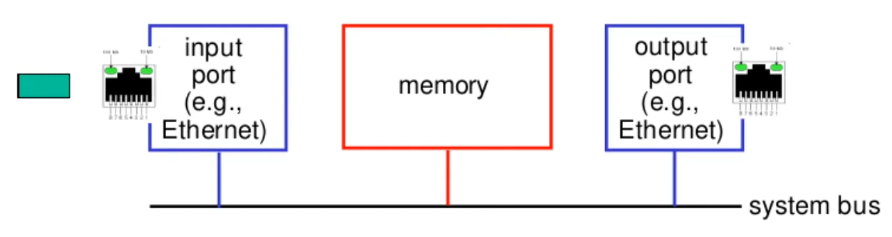
\includegraphics[width=0.65\textwidth]{img/cap-04/matriz-de-comutacao-memoria.png}
                \end{center}

                \item \textbf{Barramento :} \\
                    $\hookrightarrow$ Datagrama sai da porta de entrada para a porta de saída por um barramento compartilhado \\
                    $\hookrightarrow$ Contenção do Barramento : Limitação de velocidade pela banda do barramento. \\
                    $\hookrightarrow$ Restrição de contenção do barramento, uma vez que tem um pacote trafegando no barramento ninguem pode mais trafegar 
            
                    \begin{center}
                        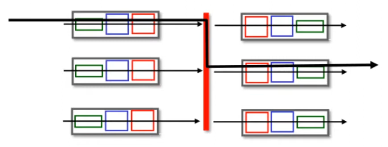
\includegraphics[width=0.65\textwidth]{img/cap-04/matriz-de-comutacao-barramento.png}
                    \end{center}

                \item \textbf{Interconexão :} \\
                    $\hookrightarrow$ Barra cruzada: série de barramentos interconectados, permitindo algum nível de paralelismo; \\
                    $\hookrightarrow$ Continua ocorrendo contenção
                    
                    \begin{center}
                        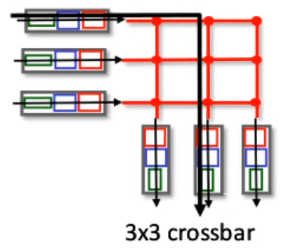
\includegraphics[width=0.55\textwidth]{img/cap-04/barra-cruzada.png}
                    \end{center}

                \item Comutação em múltiplos estágios: consiste em switches \(n \times n\) compostos por vários estágios, estruturados como uma interconexão de matrizes de comutação menores. \\
                    $\hookrightarrow$ Permite níveis de paralelismo. \\
                    $\hookrightarrow$ Fragmenta o datagrama em células de tamanho fixo, possibilitando a paralelização do envio dessas células. \\
                    $\hookrightarrow$ Comuta as células através da matriz de comutação e remonta os datagramas na saída.
                
                    \begin{center}
                        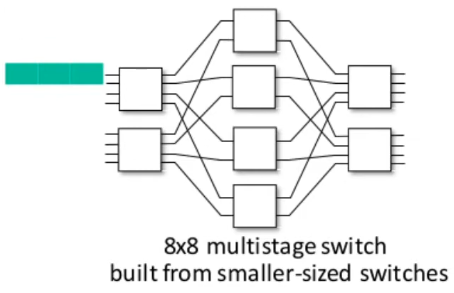
\includegraphics[width=0.65\textwidth]{img/cap-04/comutacao-em-multiplos-estagios.png}
                    \end{center}

                \item É possível escalar esse processo ainda mais parelizando as matrizes de comuração
                
                    \begin{center}
                        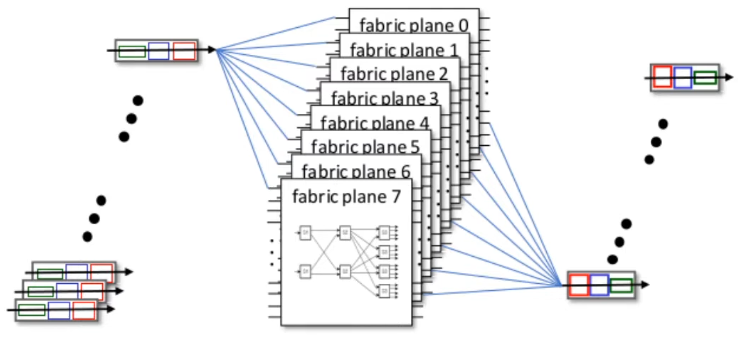
\includegraphics[width=0.65\textwidth]{img/cap-04/multiplos-estagios-escalavel.png}
                    \end{center}
            
            \end{itemize}

        \subsubsection*{Enfileiramento em Interfaces}    

            \begin{itemize}[left=0.5cm, align=left, nosep]
                \item Enfileramento na interface de entrada \\
                    $\hookrightarrow$ Se a matriz de comutação é mais lenta do que as portas de entrada combinadas $\rightarrow$ enfileramento ocorrerá na entrada de filas. \\
                    $\hookrightarrow$ Head of Lines (HOL) blocking : um datagrama enfileirado na frente da fila previne outros na fila de moverem para frente.     

                    \begin{center}
                        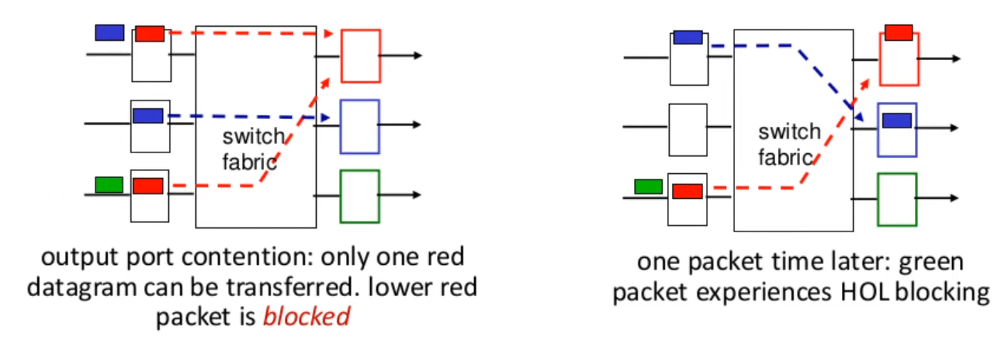
\includegraphics[width=0.65\textwidth]{img/cap-04/hol.png}
                    \end{center}

                \item Enfileramento na interface de saida \\
                    $\hookrightarrow$ Buffering (Descarte): É necessario quando datagramas chegam da matriz de comutação mais rápidos do que a taxa de transmissao do enlace \\
                    $\hookrightarrow$ Politica de descarte ? 
                        \begin{itemize}[left=0.5cm, align=left, nosep]
                            \item Datagramas podem ser perdidos devido ao congestionamento,falta de buffer
                        \end{itemize}
                    $\hookrightarrow$ Disciplinas de escalonamento : formas de lidar com a organização dos pacotes nessa fila de interface de saida para permitir priorizar trafego ou eventualmente reduzir o impacto do infileiramento na comunicação fim a fim     
                       
                    \begin{center}
                        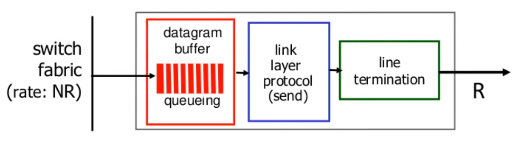
\includegraphics[width=0.65\textwidth]{img/cap-04/enfileiramento-interface-saida.png}
                    \end{center}

                    \begin{center}
                        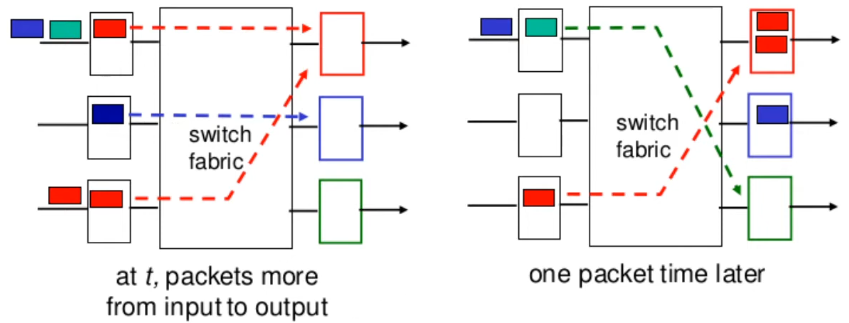
\includegraphics[width=0.65\textwidth]{img/cap-04/enfileiramento-interface-saida2.png}
                    \end{center}

                    $\hookrightarrow$ Descarte quando a taxa de chegada via switch excede a velocidade de linha de saida \\
                    $\hookrightarrow$ Enfileiramento (atraso) e a perda devida o overflow(transbordo) do buffer da porta de saida

                    $\hookrightarrow$ \textbf{Quanto de memoria é preciso se alocada para essa fila ?}
                        \begin{itemize}[left=0.5cm, align=left, nosep]
                            \item RFC 3429 : quantidade de buffer necessario para alocar será RTT vezes a capacidade do enlace C.
                            \item Recomendações recentes : com $n$ fluxos, $buffering = RTT * C / \sqrt{N}$
                            \item Porém muito buffer pode causar atraso (praticularmente em roteadores domesticos)
                            \begin{itemize}[left=0.5cm, align=left, nosep]
                                \item RTTs longos : desempenho ruim para aplicações de tempo real,
                                \item recordar que o atraso baseado no controle de congestionamento  
                            \end{itemize}
                        \end{itemize}
    
                \item Manejamento do Buffer (AQM) \\
                     $\hookrightarrow$ Gerenciar o uso das filas \\
                     $\hookrightarrow$ Descarte : qual pacote adicionar, e qual descarta quando o buffer está cheio 
                        \begin{itemize}[left=0.5cm, align=left, nosep]
                            \item Descarta da cauda : descarta pacote chegando
                            \item Prioridade : descartar/remover baseado em uma prioridade 
                        \end{itemize}    
                    
                    $\hookrightarrow$ Marcação : qual pacotes marcar para sinalixar um congestionamento (ECN,RED)

                    \begin{center}
                        \includegraphics[width=0.35\textwidth]{img/cap-04/manejamento-buffer.png}
                    \end{center}
               
            \end{itemize}
            
        \subsubsection*{Pacotes de Escalonamento :}
            \begin{itemize}[left=0.5cm, align=left, nosep]
                \item Decidir qual o proximo pacote que sera transmitido no enlace
                
                \item \textbf{FCFS} (Firt Come,FIrst Server): Pacotes são transmitidos em ordem atraves da porta de saida \\
                    $\hookrightarrow$ FIFO

                \item \textbf{Prioridade} : \\
                    $\hookrightarrow$ Classifica os pacotes chegados enfileirado-os em classes de acordo com a prioridade.
                        \begin{itemize}[left=0.5cm, align=left, nosep]
                            \item Qualquer campo do cabeçalho pode ser usado para a classificação
                        \end{itemize}    
                    $\hookrightarrow$ Envia pacotes com maiores prioridade na fila que tem pacotes bufferizados     
                        \begin{itemize}[left=0.5cm, align=left, nosep]
                            \item FCFS sem a classe de prioridade
                        \end{itemize}  

                    \begin{center}
                        \includegraphics[width=0.45\textwidth]{img/cap-04/prioridade.png}
                    \end{center}
               
                \item \textbf{Round Robin} : \\
                    $\hookrightarrow$ Classifica os pacotes chegados enfileirado-os em classes de acordo com a prioridade. 
                        \begin{itemize}[left=0.5cm, align=left, nosep]
                            \item Qualquer campo do cabeçalho pode ser usado para a classificação
                        \end{itemize}      
                    $\hookrightarrow$ Servidor ciclicamente,repetidamente escaneia as classes de filas, enviando um pacote completo de cada cada classe(se necessário) a cada turno. 
                    
                    \begin{center}
                        \includegraphics[width=0.65\textwidth]{img/cap-04/round-robin.png}
                    \end{center}
                    
                \item \textbf{Weighted Fair Queues} (WFQ) : \\
                    $\hookrightarrow$ Generalização para o round robin \\
                    $\hookrightarrow$ Cada classe,$i$, tem um peso, $W_i$, e recebe uma quantidade ponderada de serviço em cada ciclo
                        \[
                            \frac{w_i}{\sum_{j}^{} w_j}  
                        \]    
                    
                    $\hookrightarrow$ Banda minima garantida para as classes de baixa prioridade 
                    
                    \begin{center}
                        \includegraphics[width=0.65\textwidth]{img/cap-04/wfq.png}
                    \end{center}
            
            \end{itemize} 

    \subsection{IP: Internet Protocol}
    
        \begin{itemize}[left=0.5cm, align=left, nosep]
            \item Protocolo \texttt{IP} : Define a padronização para troca de informações na camada de rede da Internet:
            \begin{itemize}[left=0.5cm, nosep, label=$\hookrightarrow$]
                \item Formato do datagrama
                \item Endereçamento
                \item Convenções para tratamento de pacotes
            \end{itemize}
            \item Protocolo \texttt{ICMP} : Trata da sinalização e troca de informações de controle na rede:
            \begin{itemize}[left=0.5cm, nosep, label=$\hookrightarrow$]
                \item Reporta erros
                \item Transporta informações de sinalização
            \end{itemize}
        \end{itemize}


        \begin{itemize}[left=0.5cm, align=left, nosep]
            \item Módulos da Camada de Rede
        \end{itemize}

        \begin{center}
            \includegraphics[width=0.45\textwidth]{img/cap-04/modulos-camada-de-rede.png}
        \end{center}

        \subsubsection*{Formato do Datagrama}

            \begin{center}
                \includegraphics[width=0.45\textwidth]{img/cap-04/formato-datagrama.png}
            \end{center}

        \subsubsection*{Endereçamento}
           
            \begin{itemize}[left=0.5cm, align=left, nosep]
                \item \textbf{Endereço IP}: Identificador de 32 bits associado a cada \underline{interface} de um sistema final (host) ou roteador.  
                \begin{itemize}[left=0.5cm, nosep, label=$\hookrightarrow$]
                    \item Uma máquina com \(n\) interfaces possui \(n\) endereços IP.
                    \item Um mesmo host pode ter múltiplos endereços IP.
                \end{itemize}

                \item \textbf{Interface}: Conexão entre sistemas finais/roteadores e a camada de enlace.  
                \begin{itemize}[left=0.5cm, nosep, label=$\hookrightarrow$]
                    \item Roteadores tipicamente possuem múltiplas interfaces.
                    \item Sistemas finais, uma ou duas interfaces.
                    \item Exemplos: rede sem fio (Wi-Fi), rede móvel (4G/5G), Bluetooth.
                \end{itemize}

                \begin{center}
                    \includegraphics[width=0.45\textwidth]{img/cap-04/introducao-endereco-ip.png}
                \end{center}

                \item \textbf{Formato do Endereço IP}:  
                \begin{itemize}[left=0.5cm, nosep, label=$\hookrightarrow$]
                    \item Organizado em quatro porções de 8 bits.
                    \item Representado na forma decimal com pontos separando cada octeto (ex: \texttt{192.168.0.1}).
                \end{itemize}

                \[
                    \textbf{223.1.1.1}
                    =
                    \underbrace{11011111}_{223} \;
                    \underbrace{00000001}_{1} \;
                    \underbrace{00000001}_{1} \;
                    \underbrace{00000001}_{1}
                \]
            
            \end{itemize}

            \textbf{Sub-redes}

                \begin{itemize}[left=0.5cm, align=left, nosep]
                    \item Conjunto de interconexões que vinculam sistemas finais e interfaces de roteadores.
                    \item Dispositivos que se conectam fisicamente sem precisar de um roteador intermediário pertencem à mesma sub-rede.
                    \item Exemplo: Rede composta por três sub-redes.

                    \begin{center}
                        \includegraphics[width=0.45\textwidth]{img/cap-04/introducao-endereco-ip.png}
                    \end{center}

                    \item \textbf{Estrutura do Endereço IP :}
                    \begin{itemize}[left=0.5cm, nosep, label=$\hookrightarrow$]
                        \item Parte da sub-rede: bits mais significativos, comuns aos dispositivos da mesma rede.
                        \item Parte do hospedeiro: bits menos significativos, distintos em cada interface.
                    \end{itemize}

                    \item \textbf{Definição de sub-redes :}
                    \begin{itemize}[left=0.5cm, nosep, label=$\hookrightarrow$]
                        \item Desvincula cada interface do host/roteador, criando “ilhas” ou redes isoladas.
                        \item Cada uma dessas redes é chamada de sub-rede.
                    \end{itemize}

                    \begin{center}
                        \includegraphics[width=0.45\textwidth]{img/cap-04/sub-redes.png}
                    \end{center}

                    \item \textbf{Padrões de endereçamento :}
                    \begin{itemize}[left=0.5cm, nosep, label=$\hookrightarrow$]
                        \item Bits do hospedeiro todos 0 $\rightarrow$ endereço da sub-rede.
                        \item Bits do hospedeiro todos 1 $\rightarrow$ endereço de broadcast (datagrama enviado a todas as interfaces da sub-rede).
                    \end{itemize}

                    \begin{center}
                        \includegraphics[width=0.45\textwidth]{img/cap-04/sub-redes2.png}
                    \end{center}
                
                \end{itemize}
                            
            \textbf{CIDR (Classless Inter-Domain Routing)}

            \begin{itemize}[left=0.5cm, align=left, nosep]
                \item Permite definir sub-redes com máscaras de tamanho arbitrário, sem as restrições das classes A, B e C. 
                \item Representação: \texttt{a.b.c.d/x}, onde \(x\) indica quantos dos bits mais significativos pertencem à parte da rede (prefixo).
                \item Exemplo: o endereço \texttt{192.168.10.0/24} indica que os 24 bits iniciais identificam a rede.
            \end{itemize}

            \begin{center}
                \includegraphics[width=0.45\textwidth]{img/cap-04/cidr.png}
            \end{center}

        \subsubsection*{Como conseguir um endereço IP?}

            \textbf{Existem, na verdade, duas questões:}
            \begin{enumerate}
                \item Como um sistema final consegue um endereço IP dentro de uma rede? --> O sistema faz parte da rede.
                \item Como uma rede obtém um endereço IP? --> A rede faz parte do endereço.
            \end{enumerate}

            \textbf{Como um sistema final consegue um endereço IP?}
            \begin{itemize}[left=0.5cm, align=left, nosep]
                \item Configuração manual : Administradores configuram manualmente o endereço nos arquivos da interface de rede.
                \item DHCP (Dynamic Host Configuration Protocol) : Obtém dinamicamente endereços de um servidor.
                    \begin{itemize}[left=0.5cm, nosep, label=$\hookrightarrow$]
                        \item Plug and play  
                    \end{itemize} 
            \end{itemize}

            \textbf{DHCP (Dynamic Host Configuration Protocol)}
            \begin{itemize}[left=0.5cm, align=left, nosep]
                \item Objetivo : Sistema final obtém dinamicamente um endereço IP ao entrar na rede.
                \item Protocolo de aplicação baseado em UDP.
                    \begin{itemize}[left=0.5cm, nosep, label=$\hookrightarrow$]
                        \item Pode renovar o endereço reservado.
                        \item Permite reutilização de endereços.
                        \item Oferece suporte a usuários móveis que entram e saem da rede.
                    \end{itemize} 
                \item Visão geral $\rightarrow$ Processo de comunicação entre cliente e servidor DHCP :
                    \begin{itemize}[left=0.5cm, nosep, label=$\hookrightarrow$]
                        \item Sistema final envia uma mensagem em broadcast para descobrir servidores DHCP disponíveis [DHCP Discover].
                        \item Servidor responde com mensagem \texttt{DHCP Offer}.
                        \item Sistema final solicita o endereço IP $\rightarrow$ mensagem \texttt{DHCP Request}.
                        \item Servidor confirma o endereço $\rightarrow$ mensagem \texttt{DHCP ACK}.
                    \end{itemize}
            \end{itemize}

            \begin{center}
                \includegraphics[width=0.45\textwidth]{img/cap-04/dhcp.png}
            \end{center}

            \texttt{Broadcast universal} : Todos os bits do endereço IP configurados com 1 (255.255.255.255).

            \begin{center}
                \includegraphics[width=0.45\textwidth]{img/cap-04/dhcp2.png}
            \end{center}

            \begin{itemize}[left=0.5cm, align=left, nosep]
                \item DHCP pode fornecer informações adicionais além do endereço IP :
                    \begin{itemize}[left=0.5cm, nosep, label=$\hookrightarrow$]
                        \item Endereço do primeiro salto (roteador padrão).
                        \item Nome e endereço IP do servidor DNS.
                        \item Máscara da sub-rede : Usada para determinar os limites da rede e a porção de endereçamento IP destinada aos dispositivos locais.
                    \end{itemize}    
                \end{itemize}

            \begin{center}
                \includegraphics[width=0.45\textwidth]{img/cap-04/dhcp-exemplo.png}
            \end{center}

            \begin{center}
                \includegraphics[width=0.45\textwidth]{img/cap-04/dhcp-exemplo2.png}
            \end{center}


            \textbf{Como uma rede obtém um endereço IP ?}
            \begin{itemize}[left=0.5cm, align=left, nosep]
                \item Cada sub-rede recebe um bloco de endereços a partir de um provedor de acesso à Internet (ISP).
                
                \[
                    \textbf{Bloco do ISP:} \quad
                    \uline{11001000 \; 00010111 \; 00010000} \; 00000000
                    \quad 200.23.16.0/20
                \]
                
                \item ISPs podem dividir esse bloco em sub-blocos menores.
            \end{itemize}

            \begin{center}
                \begin{tabular}{l l l l l l}
                    \textbf{Organization 0} & 11001000 & 00010111 & 00010000 & 00000000 & 200.23.16.0/23 \\
                    \textbf{Organization 1} & 11001000 & 00010111 & 00010010 & 00000000 & 200.23.18.0/23 \\
                    \textbf{Organization 2} & 11001000 & 00010111 & 00010100 & 00000000 & 200.23.20.0/23 \\
                    \textbf{...}            & .....    & .....    & .....    & ....     & \\
                    \textbf{Organization 7} & 11001000 & 00010111 & 00011110 & 00000000 & 200.23.30.0/23 \\
                \end{tabular}
            \end{center}

            \subsubsection*{Endereçamento Hierárquico}
            \begin{itemize}[left=0.5cm, align=left, nosep]
                \item O endereçamento hierárquico permite divulgação eficiente de informações de roteamento (agregação de rotas).
            \end{itemize}

            \begin{center}
                \includegraphics[width=0.45\textwidth]{img/cap-04/hierarquia-de-endereco.png}
            \end{center}

            \begin{itemize}[left=0.5cm, align=left, nosep]
                \item Quando uma organização troca de provedor, o endereço pode ser mantido.
                \item O roteamento usa o casamento de maior prefixo (rotas específicas).
            \end{itemize}

            \begin{center}
                \includegraphics[width=0.45\textwidth]{img/cap-04/endereco-hierarquico.png}
            \end{center}

        \subsubsection*{Endereçamento de IP : Últimos Comentários}
            \textbf{Como um ISP consegue um bloco de endereços ?}
            \begin{itemize}[left=0.5cm, align=left, nosep]
                \item ICANN (Internet Corporation for Assigned Names and Numbers) : Responsável por alocar blocos de endereços IP a grandes provedores.
                    \begin{itemize}[left=0.5cm, nosep, label=$\hookrightarrow$]
                        \item Coordena cinco registros regionais (RIRs).
                        \item Administra os servidores raiz do DNS.
                        \item Gerencia a delegação de domínios de topo (TLDs), como \texttt{.com}, \texttt{.edu}, etc.
                    \end{itemize}     
            \end{itemize}

            \textbf{Temos endereços IPv4(IP 32-bits) suficientes?}
            \begin{itemize}[left=0.5cm, align=left, nosep]
                \item A ICANN alocou o último bloco de endereços IPv4 em 2011.
                \item NAT prolonga a utilização do espaço IPv4.
                \item IPv6 possui espaço de endereçamento de 128 bits.
            \end{itemize}
    
        \subsubsection*{NAT: Network Address Translation}

            \begin{itemize}[left=0.5cm, align=left, nosep]
                \item Todos os dispositivos em uma rede local compartilham \underline{apenas um} endereço IPv4 do ponto de vista da Internet.

                \begin{center}
                    \includegraphics[width=0.45\textwidth]{img/cap-04/nat.png}
                \end{center}

                \item Dispositivos em uma rede local possuem um espaço de endereçamento IP privado de 32 bits, prefixos 10/8, 172.16/12 e 192.168/16 (válido apenas dentro da rede local).

                \item Vantagens : 
                \begin{itemize}[left=0.5cm, nosep, label=$\hookrightarrow$]
                    \item Apenas um endereço público é suficiente para todos os dispositivos internos.  
                    \item Mudança de endereços internos sem necessidade de informar a rede externa.  
                    \item Troca de provedor de Internet sem impacto no espaço interno.  
                    \item Segurança : Dispositivos internos não são diretamente acessíveis externamente.
                \end{itemize}     
                
                \item Implementação : Ocorre na borda da rede.
                \begin{itemize}[left=0.5cm, nosep, label=$\hookrightarrow$]
                    \item Datagramas de saída : substitui (endereço IP de origem, número da porta) por (endereço válido do NAT, novo número de porta)
                        \begin{itemize}[left=0.5cm, nosep, label=$-$]
                            \item Clientes e servidores externos respondem a esse novo par.
                        \end{itemize}
                    \item A tabela NAT mapeia (endereço IP de origem, número da porta) para (endereço NAT, nova porta). 
                    \item Datagramas de entrada : Realiza o processo inverso, substituindo (endereço NAT, nova porta) por (endereço interno, porta original).  
                \end{itemize}

                \begin{center}
                    \includegraphics[width=0.45\textwidth]{img/cap-04/nat2.png}
                \end{center}

                \item NAT é controverso
                \begin{itemize}[left=0.5cm, nosep, label=$\hookrightarrow$]
                    \item Roteadores deveriam operar apenas até a camada 3.
                    \item A escassez de endereços deveria ser resolvida pelo IPv6.
                    \item Viola o princípio fim-a-fim (endereços e portas são modificados pela camada de rede).
                    \item Atravessar NAT : Como um cliente externo se conecta a um servidor atrás do NAT ?
                \end{itemize}    

                \item Apesar disso, NAT continua amplamente usado :
                \begin{itemize}[left=0.5cm, nosep, label=$\hookrightarrow$]
                    \item Presente em redes domésticas, institucionais e em infraestruturas 4G/5G.
                \end{itemize}  
            
            \end{itemize}

        \subsubsection*{IPv6}
            \begin{itemize}[left=0.5cm, align=left, nosep]
                \item \textbf{Motivação inicial} : O espaço de endereçamento IPv4 (32 bits) foi completamente alocado.
                \item \textbf{Motivação adicional} :
                \begin{itemize}[left=0.5cm, nosep, label=$\hookrightarrow$]
                    \item Maior velocidade de processamento e encaminhamento, cabeçalho fixo de 40 bytes.  
                    \item Permite diferentes tratamentos de fluxo na camada de rede.
                \end{itemize}     
                
                \item Formato do datagrama IPv6
                \begin{center}
                    \includegraphics[width=0.4\textwidth]{img/cap-04/ipv6-formato}
                \end{center}

                \item Diferenças em relação ao IPv4 :
                \begin{itemize}[left=0.5cm, nosep, label=$\hookrightarrow$]
                    \item Sem campo de checksum (reduz o custo de processamento nos roteadores).  
                    \item Sem fragmentação ou remontagem de datagramas.  
                    \item Sem campo de opções, controle feito pelo cabeçalho de extensão (next header).
                \end{itemize} 

            \end{itemize}

        \subsubsection*{Transição do IPv64 para o IPv6}
            \begin{itemize}[left=0.5cm, align=left, nosep]
                \item Nem todos os roteadores podem ser atualizados simultaneamente
                
                \begin{itemize}[left=0.5cm, nosep, label=$\hookrightarrow$]
                    \item Sem “flag days” (substituição coletiva).  
                    \item Como a Internet lida com roteadores operando IPv4 e IPv6 simultaneamente?
                \end{itemize}     

                \item Tunelamento : Datagrama IPv6 encapsulado dentro de um datagrama IPv4 entre roteadores IPv4 (pacotes dentro de pacotes). 
                \begin{itemize}[left=0.5cm, nosep, label=$\hookrightarrow$]
                    \item Técnica usada também em outros contextos, como redes 4G/5G.
                \end{itemize} 

                \begin{center}
                    \includegraphics[width=0.4\textwidth]{img/cap-04/tunelamento.png}
                \end{center}

                \begin{center}
                    \includegraphics[width=0.4\textwidth]{img/cap-04/tunelamento-encapsulamento.png}
                \end{center}

                \begin{center}
                    \includegraphics[width=0.4\textwidth]{img/cap-04/tunelamento-encapsulamento2.png}
                \end{center}

                \begin{center}
                    \includegraphics[width=0.4\textwidth]{img/cap-04/tunelamento2.png}
                \end{center}

                \item Adoção do IPv6 : 
                \begin{itemize}[left=0.5cm, nosep, label=$\hookrightarrow$]
                    \item Google : 30\% dos clientes acessam via IPv6
                    \item NIST : Cerca de $\frac{1}{3}$ dos domínios do governo dos EUA têm suporte a IPv6.  
                    \item Processo de migração LONGO!! 
                    \begin{itemize}[left=0.5cm, nosep, label=$-$]
                        \item Mais de 25 anos 
                        \item Comparação: mudanças drásticas na camada de aplicação (WWW, redes sociais, streaming, jogos etc.).           
                    \end{itemize} 
                \end{itemize}    
                
                \begin{center}
                    \includegraphics[width=0.4\textwidth]{img/cap-04/adocao-ipv6.png}
                \end{center}

            \end{itemize}           
            
            %\begin{itemize}[left=0.5cm, align=left, nosep]
            %    \item \\
            %    \begin{itemize}[left=0.5cm, nosep, label=$\hookrightarrow$]
            %        \item \\
            %    \end{itemize}     
            %\end{itemize}


    \subsection{MiddleBox}


\section{Camada de Enlace}


\end{document}
